%===============================================================================
% LaTeX sjabloon voor de bachelorproef toegepaste informatica aan HOGENT
% Meer info op https://github.com/HoGentTIN/bachproef-latex-sjabloon
%===============================================================================

\documentclass{bachproef-tin}

\usepackage{hogent-thesis-titlepage} % Titelpagina conform aan HOGENT huisstijl

%%---------- Documenteigenschappen ---------------------------------------------
% TODO: Vul dit aan met je eigen info:

% De titel van het rapport/bachelorproef
\title{Personalized Search: Graph vs. OLAP Database}

% Je eigen naam
\author{Shauni Van de Velde}

% De naam van je promotor (lector van de opleiding)
\promotor{Guy Dekoning}

% De naam van je co-promotor. Als je promotor ook je opdrachtgever is en je
% dus ook inhoudelijk begeleidt (en enkel dan!), mag je dit leeg laten.
\copromotor{Nicolas Lierman}

% Indien je bachelorproef in opdracht van/in samenwerking met een bedrijf of
% externe organisatie geschreven is, geef je hier de naam. Zoniet laat je dit
% zoals het is.
\instelling{MultiMinds}

% Academiejaar
\academiejaar{2019-2020}

% Examenperiode
%  - 1e semester = 1e examenperiode => 1
%  - 2e semester = 2e examenperiode => 2
%  - tweede zit  = 3e examenperiode => 3
\examenperiode{2}

%===============================================================================
% Inhoud document
%===============================================================================

\begin{document}

%---------- Taalselectie -------------------------------------------------------
% Als je je bachelorproef in het Engels schrijft, haal dan onderstaande regel
% uit commentaar. Let op: de tekst op de voorkaft blijft in het Nederlands, en
% dat is ook de bedoeling!

%\selectlanguage{english}

%---------- Titelblad ----------------------------------------------------------
\inserttitlepage

%---------- Samenvatting, voorwoord --------------------------------------------
\usechapterimagefalse
%%=============================================================================
%% Voorwoord
%%=============================================================================

\chapter*{\IfLanguageName{dutch}{Woord vooraf}{Preface}}
\label{ch:voorwoord}

%% TODO:
%% Het voorwoord is het enige deel van de bachelorproef waar je vanuit je
%% eigen standpunt (``ik-vorm'') mag schrijven. Je kan hier bv. motiveren
%% waarom jij het onderwerp wil bespreken.
%% Vergeet ook niet te bedanken wie je geholpen/gesteund/... heeft


%%=============================================================================
%% Samenvatting
%%=============================================================================

% TODO: De "abstract" of samenvatting is een kernachtige (~ 1 blz. voor een
% thesis) synthese van het document.
%
% Deze aspecten moeten zeker aan bod komen:
% - Context: waarom is dit werk belangrijk?
% - Nood: waarom moest dit onderzocht worden?
% - Taak: wat heb je precies gedaan?
% - Object: wat staat in dit document geschreven?
% - Resultaat: wat was het resultaat?
% - Conclusie: wat is/zijn de belangrijkste conclusie(s)?
% - Perspectief: blijven er nog vragen open die in de toekomst nog kunnen
%    onderzocht worden? Wat is een mogelijk vervolg voor jouw onderzoek?
%
% LET OP! Een samenvatting is GEEN voorwoord!

%%---------- Nederlandse samenvatting -----------------------------------------
%
% TODO: Als je je bachelorproef in het Engels schrijft, moet je eerst een
% Nederlandse samenvatting invoegen. Haal daarvoor onderstaande code uit
% commentaar.
% Wie zijn bachelorproef in het Nederlands schrijft, kan dit negeren, de inhoud
% wordt niet in het document ingevoegd.

\IfLanguageName{english}{%
\selectlanguage{dutch}
\chapter*{Samenvatting}
\lipsum[1-4]
\selectlanguage{english}
}{}

%%---------- Samenvatting -----------------------------------------------------
% De samenvatting in de hoofdtaal van het document

\chapter*{\IfLanguageName{dutch}{Samenvatting}{Abstract}}

In samenwerking met MultiMinds werd besloten onderzoek te voeren naar de haalbaarheid van het gebruik van twee vooraf bepaalde opties voor het implementeren van een gepersonaliseerde zoekfunctie bij e-commerce toepassingen, de  opties die gekozen werden door de opdrachtgever zijn Neo4j en Elasticsearch.  

De reden voor dit onderzoek is dat zo goed als alle gekende webshops gebruik maken van een zoekfunctie, maar dat deze vaak beperkt blijft tot de productcatalogus. In dit onderzoek wordt dus nagegaan of het mogelijk is deze zoekfunctie uit te breiden met data van gebruikers om zo een meer gepersonaliseerd resultaat te kunnen opleveren.

Enkele voorbeelden van dergelijke gebruikersdata zijn geslacht, leeftijd, locatie, etc., maar ook bijvoorbeeld familiale verbanden. Zo is het bijvoorbeeld wenselijk dat in het geval van twee samenwonenden, Persoon A en persoon B, er merken worden aanbevolen aan Persoon A waarvan Persoon B regelmatig producten koopt.

In eerste instantie werd er een literatuurstudie gedaan naar de reeds bestaande vormen van personalisatie, al dan niet binnen e-commerce toepassingen als marketingvorm.

Ten tweede werden de verschillende types van aanbevelingssystemen onderzocht. Daarbij werden twee belangrijke families gevonden: Collaborative Filtering-algoritmen, en Content Based-algoritmen. Voor de implementatie van dergelijke algoritmen zijn ook hybride vormen mogelijk, deze hybride vormen werden gebruikt in dit onderzoek.

Ten derde werd er ook een literatuuronderzoek gedaan naar de twee platformen, Neo4j en Elasticsearch. In dit deel van het onderzoek werd bekeken of deze platformen de mogelijkheden hadden om een aanbevelingssysteem te implementeren dat voldoende accurate resultaten zou opleveren. Uit dit onderzoek bleek dat Neo4j sterk uitblinkt in het gebruiken van data over de relaties tussen twee personen, waar Elasticsearch eerder uitblinkt in het zeer snel opleveren van resultaten die aan bepaalde criteria voldoen.

Als vierde puntje in het onderzoek werd ook verder ingegaan op een nadeel dat het personaliseren van e-commerce toepassingen met zich mee kan brengen, namelijk een 'Filter Bubble', waarbij gebruikers enkel nog resultaten te zien krijgen die volledig passen bij hun profiel. Bijgevolg zullen gebruikers weinig of zelfs geen resultaten mogen verwachten die door hun nog niet gezien werden.

Als laatste deel van de literatuurstudie werd bekeken of de implementatie van een systeem dat op deze manier gebruik maakt van persoonlijke data en gegevens wel als legaal aanschouwd kan worden onder de wetgeving van de GDPR. Onderzoek wees uit dat het systeem hier geen problemen van zou mogen ondervinden.

De resultaten van dit onderzoek wezen uit dat beide platformen hun eigen voor- en nadelen met zich meebrachten, verwijzend naar de verschillende functionaliteiten die onze zoekfunctie vereist. Een belangrijke factor bij het maken van de keuze is ook de eenvoud van de implementatie, waarbij al snel bleek dat het zeer moeilijk zal is om de sterktes van Neo4j te repliceren in Elasticsearch, of omgekeerd.

De resultaten zetten aan tot verder onderzoek naar de mogelijkheid om deze twee systemen parallel te gebruiken, en de resultaten ervan te combineren.  Zo kan Neo4j gebruikt worden als een 'Knowledge Graph', die dient als aanvulling voor de data die Elasticsearch tot zijn beschikking heeft. 




%---------- Inhoudstafel -------------------------------------------------------
\pagestyle{empty} % Geen hoofding
\tableofcontents  % Voeg de inhoudstafel toe
\cleardoublepage  % Zorg dat volgende hoofstuk op een oneven pagina begint
\pagestyle{fancy} % Zet hoofding opnieuw aan

%---------- Lijst figuren, afkortingen, ... ------------------------------------

% Indien gewenst kan je hier een lijst van figuren/tabellen opgeven. Geef in
% dat geval je figuren/tabellen altijd een korte beschrijving:
%
%  \caption[korte beschrijving]{uitgebreide beschrijving}
%
% De korte beschrijving wordt gebruikt voor deze lijst, de uitgebreide staat bij
% de figuur of tabel zelf.

\listoffigures
\listoftables

% Als je een lijst van afkortingen of termen wil toevoegen, dan hoort die
% hier thuis. Gebruik bijvoorbeeld de ``glossaries'' package.
% https://www.overleaf.com/learn/latex/Glossaries

%---------- Kern ---------------------------------------------------------------

% De eerste hoofdstukken van een bachelorproef zijn meestal een inleiding op
% het onderwerp, literatuurstudie en verantwoording methodologie.
% Aarzel niet om een meer beschrijvende titel aan deze hoofstukken te geven of
% om bijvoorbeeld de inleiding en/of stand van zaken over meerdere hoofdstukken
% te verspreiden!

%%=============================================================================
%% Inleiding
%%=============================================================================

\chapter{\IfLanguageName{dutch}{Inleiding}{Introduction}}
\label{ch:inleiding}

\section{\IfLanguageName{dutch}{Probleemstelling}{Problem Statement}}
\label{sec:probleemstelling}

Elke webshop of e-commerce toepassing die vandaag de dag gekend is maakt gebruik van een zoekfunctie die gebruikers toelaat om snel en eenvoudig producten te kunnen opzoeken. Deze zoekfunctie is beperkt tot de beschikbare informatie, en bijgevolg dus in de meeste gevallen gelimiteerd tot de productcatalogus.

 Rekeninghoudend met de algemene trend rond personalisering van de \textit{customer experience } zou het ook aangewezen zijn om ook de zoekfunctionaliteit op e-commerce websites te personaliseren. Dit zou resulteren in een betere customer experience voor de klant en een hogere conversie voor het bedrijf.
 
 Het personaliseren wordt in deze context bedoeld als het gebruiken van persoonlijke data om de resultaten van een zoekopdracht te verfijnen en zo producten te kunnen aanbieden die passen bij de voorkeuren en het gedrag van de gebruiker. 
 
 Hierop biedt dit onderzoek een mogelijke oplossing om dergelijke functionaliteiten te bereiken. Er zullen twee vooraf bepaalde platformen gebruikt worden om dit uit te werken, namelijk Neo4j en Elasticsearch. Het onderzoek zal uitwijzen welk platform het meest geschikt is om een gepersonaliseerde zoekfunctie mee te implementeren.
 
  Belangrijk hierbij is om na te gaan of de wetgeving omtrent GDPR het gebruik van de persoonlijke data als legaal aanschouwt in de context van zoekfuncties, meer specifiek op welke manier deze data gebruikt zal worden binnen de uitwerking van de twee voorgenoemde platformen.


\section{\IfLanguageName{dutch}{Onderzoeksvraag}{Research question}}
\label{sec:onderzoeksvraag}

De onderzoeksvraag bestaat eruit om te ontdekken welk van de twee vooraf gekozen platformen of welke technologie de beste oplossing biedt om in real-time op grote schaal gepersonaliseerde zoekresultaten te kunnen leveren.

Belangrijke criteria hierbij zijn snelheid, performantie, kwaliteit van de resultaten, en of het al dan niet mogelijk is om familierelaties te kunnen verwerken. Met performantie wordt hier geduid op de rekenkracht die een zoekoperatie zal nodig hebben, dit is gerelateerd aan de kost. 

Nog een niet te missen detail is de invloed van de wetgeving rond GDPR, en of een gepersonaliseerde zoekfunctie op basis van persoonlijke data al dan niet als legaal wordt aanzien onder deze wetgeving.

Concreet omvat dit onderzoek volgende vier onderzoeksvragen:
\begin{itemize}
	\item Is het implementeren van een gepersonaliseerde zoekfunctie op basis van persoonlijke data legaal onder de wetgeving rond GDPR?
	\item Welke technologie biedt de mogelijkheid om een gepersonaliseerde zoekfunctie te implementeren?
	\item Welke technologie biedt de beste resultaten op basis van snelheid, performantie en kwaliteit?
	\item Laten deze technologieën toe om rekening te houden met factoren die niet te maken hebben met historisch koopgedrag (bv. leeftijd, geslacht, gezinssamenstelling)?
\end{itemize} 

Deze vragen zullen doorheen dit onderzoek een antwoord krijgen.

\section{\IfLanguageName{dutch}{Onderzoeksdoelstelling}{Research objective}}
\label{sec:onderzoeksdoelstelling}

Het onderzoek heeft als doel om te ontdekken in hoeverre de persoonlijke data van een specifieke gebruiker en contextuele data kan ingeschakeld en gecombineerd worden met de data uit een productcatalogus om persoonlijke en relevante zoekresultaten te genereren.

Dit zal verwezenlijkt worden door middel een prototype op te stellen van beide vooraf gekozen platformen, zijnde Neo4j en Elasticsearch, en de mogelijkheden ervan te ontdekken. De ondervindingen van het onderzoek, naast de informatie die een literatuurstudie biedt, zullen een antwoord geven op de onderzoeksvragen.

Bij het gebruik van contextuele data wordt hier geduid op vooral historische koopdata van de persoon zelf, maar ook demografische data zoals geslacht, leeftijd, gezinssamenstelling kunnen hierbij belangrijke factoren zijn. 

Het is niet enkel de mogelijkheid om dergelijk zoeksysteem te verwezenlijken die van belang is voor dit onderzoek, ook het gebruiksgemak en eenvoud van installatie speelt hierbij een rol, en zullen ondanks een eerder subjectieve voorwaarde te zijn toch effect hebben op de conclusie.

\section{\IfLanguageName{dutch}{Opzet van deze bachelorproef}{Structure of this bachelor thesis}}
\label{sec:opzet-bachelorproef}

% Het is gebruikelijk aan het einde van de inleiding een overzicht te
% geven van de opbouw van de rest van de tekst. Deze sectie bevat al een aanzet
% die je kan aanvullen/aanpassen in functie van je eigen tekst.

De rest van deze bachelorproef is als volgt opgebouwd:

In Hoofdstuk~\ref{ch:stand-van-zaken} wordt een overzicht gegeven van de stand van zaken binnen het onderzoeksdomein, op basis van een literatuurstudie.

In Hoofdstuk~\ref{ch:methodologie} wordt de methodologie toegelicht en worden de gebruikte onderzoekstechnieken besproken om een antwoord te kunnen formuleren op de onderzoeksvragen.

% TODO: Vul hier aan voor je eigen hoofstukken, één of twee zinnen per hoofdstuk

In Hoofdstuk~\ref{ch:conclusie}, tenslotte, wordt de conclusie gegeven en een antwoord geformuleerd op de onderzoeksvragen. Daarbij wordt ook een aanzet gegeven voor toekomstig onderzoek binnen dit domein.
\chapter{\IfLanguageName{dutch}{Stand van zaken}{State of the art}}
\label{ch:stand-van-zaken}

% Tip: Begin elk hoofdstuk met een paragraaf inleiding die beschrijft hoe
% dit hoofdstuk past binnen het geheel van de bachelorproef. Geef in het
% bijzonder aan wat de link is met het vorige en volgende hoofdstuk.

% Pas na deze inleidende paragraaf komt de eerste sectiehoofding.

\section{Personalisatie}
\label{sec:Personalisatie}

Personalisatie van webapplicaties en websites draait erom de bezoekers een op maat gemaakte ervaring aan te bieden. Dit kan op verschillende manieren toegepast worden, en kan meerdere doelen hebben. 

In dit hoofdstuk wordt er verder ingegaan op welke manieren personalisatie van websites wordt toegepast, en wat dit betekent voor zowel de bezoeker als het bedrijf zelf.

\subsection{Personalisatie op basis van e-mail en sociale media}
\label{subsec:Personalisatie op basis van e-mail en Social Media}

Zowat iedereen heeft wel te kampen met een overvloed aan e-mails in hun postvak van allerlei websites waar ze hun e-mailadres ooit hebben vrijgegeven. Het is een courante denkwijze om er van uit te gaan dat deze  e-mails door de meeste mensen simpelweg verwijderd worden, maar e-mailmarketing blijft een van de meest succesvolle marketingstrategieën \autocite{Dehkordi2012}. 

E-mailmarketing is relatief makkelijk te implementeren en vereist weinig technische investering, meestal wordt dit verwezenlijkt via systemen van derden zoals bijvoorbeeld \href{https://mailchimp.com/}{MailChimp}. 

Een nadeel van deze marketingvorm is dat het bedrijf continu bezig moet zijn met nieuwe inhoud te creëren voor deze e-mails, ook moet de website continu geüpdatet worden met relevante informatie en pagina's die relevant zijn voor de e-mails die ze versturen.

\subsection{Personalisatie op basis van geografische locatie}
\label{subsec:Personalisatie op basis van geografische locatie}

Geografische personalisatie is het aanpassen van de website op basis van de locatie van de gebruiker. Gebruikers uit België die naar de website van een internationaal bedrijf surfen, zullen dan worden omgeleid naar een Nederlandse of Franse versie van die website.

Geografische personalisatie kan ook gebruikt worden om de inhoud van een pagina aan te passen aan de hand van de locatie van de gebruiker, of om vertalingen aan te bieden.

Een nadeel hiervan is dat mensen die op reis gaan het soms moeilijk zouden kunnen hebben om naar de juiste versie van de website te navigeren, aangezien het systeem de gebruiker zal willen omleiden naar de pagina of inhoud die voorzien is voor het land waar zij zich momenteel in bevinden. Eenzelfde probleem kan zich voordoen bij bedrijven die hun webverkeer omleiden via een ander land door middel van bijvoorbeeld een VPN. 

Een mogelijke oplossing voor dit probleem is het bijhouden van cookies. Als de geografische informatie over een gebruiker daarin wordt opgeslagen, kan deze via de cookie opgehaald worden en zal een gebruiker alsnog de website met de correcte inhoud en taal aangeboden kregen. Als de gebruiker geen cookies toelaat, of zijn cookies verwijdert, wordt deze mogelijke oplossing tenietgedaan.

Geografische personalisatie is ook relatief eenvoudig te implementeren en kan een grote troef zijn op de internationale markt. 

\subsection{Personalisatie op basis van IP-adres}
\label{subsec:Personalisatie op basis van IP-adres}

Deze methode van personalisatie is wat minder opvallend, aangezien het bij de gemiddelde internetgebruiker weinig tot nooit zal voorkomen, dit omdat zij het internet gebruiken via een serviceprovider zoals Telenet of Proximus. 

Deze vorm van personalisatie wordt gebruikt om zakelijke gebruikers en bedrijven te kunnen identificeren op basis van hun IP-adres. Zo kan men zien of een bezoeker bij een bepaald bedrijf werkzaam is om deze direct aan te spreken op bijvoorbeeld de homepagina.

	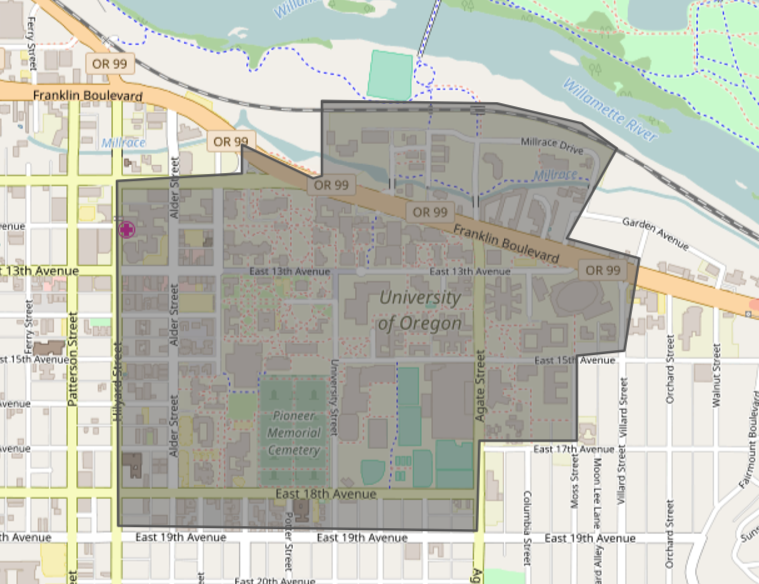
\includegraphics[width=\linewidth]{img/e2fcfe784532c41a644e4465f535530d}

Net zoals bij personalisatie op basis van locatie kan dit misleidende resultaten opleveren, bijvoorbeeld als de werknemer van thuis werkt of het IP-adres niet duidelijk aantoont vanuit welk bedrijf het webverkeer van de bezoeker afkomstig is. Ook voor performantie kan dit negatieve gevolgen hebben, aangezien deze vorm van personalisatie afhankelijk is van systemen van derden. 

Verder moet er ook inhoud gecreëerd worden voor elk bedrijf dat men specifiek wil aanspreken. Dit is een tijdrovend proces, maar aangezien deze vorm van personalisatie weinig voorkomt, is het wel een troef waardoor het bedrijf zich kan onderscheiden van de meerderheid en zich kan laten opvallen.

  
 \subsection{Verwante inhoud personalisatie}
 \label{subsec:Verwante inhoud personalisatie}
 
 Dit is de vorm van personalisatie die een grote meerwaarde zal leveren aan dit onderzoek. De meeste mensen hebben deze vorm al ondervonden op een webshop zoals Amazon of Bol.com. Deze vorm van personalisatie draait erom de gebruikers artikels of producten aan te raden op basis van items die ze al eerder bekeken hebben, alsook het gedrag van andere gebruikers.
 
De werking van het aanbevelingssysteem van Amazon is gebaseerd op enkele complexe algoritmen. \autocite{Linden2003} Dit is natuurlijk verantwoord omdat zij een gigant zijn in de e-commerce industrie. Amazon werkt op zeer grote schaal werken en heeft veel geld geïnvesteerd in de ontwikkeling van hun systeem. 

In de realiteit hoeven de technologieën voor aanbevelingen van producten niet zo complex te zijn voor gewone webshops en bedrijven, vaak is het voldoende om relaties te creëren tussen artikels en op basis van deze relaties nieuwe artikels aan te raden aan de gebruikers. 

Een voorbeeld van een relatie tussen twee artikels is de welbekende 'Anderen bekeken ook' blok die vaak zichtbaar is bij het bekijken van een detailpagina van een product. 

Een simpelere methode van dergelijke relaties is het aanbieden van verwante producten op basis van categorieën of tags. Tags zijn een manier om kenmerken van een product weer te geven die specifieker zijn dan een categorie. Een categorie kan dan 'schoenen' zijn, terwijl een tag 'lage sneakers' is. 

Dit is een klassiek voorbeeld van de probleemstelling van dit onderzoek. De zoekfunctie is dus beperkt tot de productcatalogus en de informatie die beschikbaar is over deze producten. De website maakt dus geen gebruik van persoonlijke informatie om deze zoekresultaten te personaliseren.

Over de mogelijkheden van het personaliseren van zoekresultaten gaan we dieper in in het volgende hoofdstuk van deze literatuurstudie.

\section{Recommender Systems}
\label{sec:Recommender Systems}
Recommender Systems \autocite{Resnick1997} zijn aanbevelingen vanuit het systeem die rekening houden met de beschikbare informatie van gebruikers en hun voorkeuren om zo een filter te plaatsen op de informatie die weergegeven wordt. Verder zullen we deze benoemen aan de hand  van hun Nederlandse naam 'aanbevelingssystemen'.

Aanbevelingssystemen worden vooral gebruikt in een e-commerce toepassingen waar een zeer groot en verscheiden aanbod aan producten is, en het al vaak lastig wordt om precieze aanbevelingen aan de klant te geven. Hierbij wordt allerlei informatie van een gebruiker verzameld, zoals historische aankopen, items op het verlanglijstje, items waar de gebruiker op geklikt heeft, etc.

In dit onderdeel zullen we kort wat dieper ingaan op de werking van dergelijke aanbevelingssystemen en de achterliggende algoritmen.

\subsection{Haalbaarheid}
\label{sec:Haalbaarheid}

Een degelijk systeem biedt een grote meerwaarde voor een bedrijf, zo heeft Netflix een competitie gehouden die 1 miljoen dollar bood aan degene die een aanbevelingssysteem kon maken dat 10\% beter presteerde dan hun bestaande systeem. 

Deze wedstrijd liep van oktober 2006 tot minstens oktober 2011. De wedstrijd werd de \cite{NetflixPrize} genoemd, Netflix stelde hiervoor een dataset beschikbaar. Enkele groepen hebben het doel behaald, maar het algoritme van de winnende groep is uiteindelijk nooit in productie gebracht, omdat de mogelijke opbrengst niet kon opwegen tegen de extra gevraagde rekenkracht. 

Een aanbevelingssysteem moet dus niet enkel de juiste waarden kunnen aangeven, het moet ook realistisch en haalbaar zijn qua rekenkracht en extra bijkomende kosten voor onderhoud. Het ontwerpen van dergelijk systeem is dus geen eenvoudige klus.

\subsection{Algoritmen voor aanbevelingssystemen}
\label{sec:Algoritmen voor aanbevelingssystemen}

We spreken over twee grote categorieën in algoritmen van aanbevelingssystemen: 'collaborative filtering'-algoritmen en 'content based'-algoritmen.  \autocite{Adamovicius2005} Door de evolutie en groeiende ontwikkeling van beter presterende systemen zijn er ondertussen ook enkele algoritmen die niet echt binnen een van deze twee koepels vallen. In de onderstaande figuur wordt een simpele representatie gegeven van de werking van deze soorten algoritmes.

	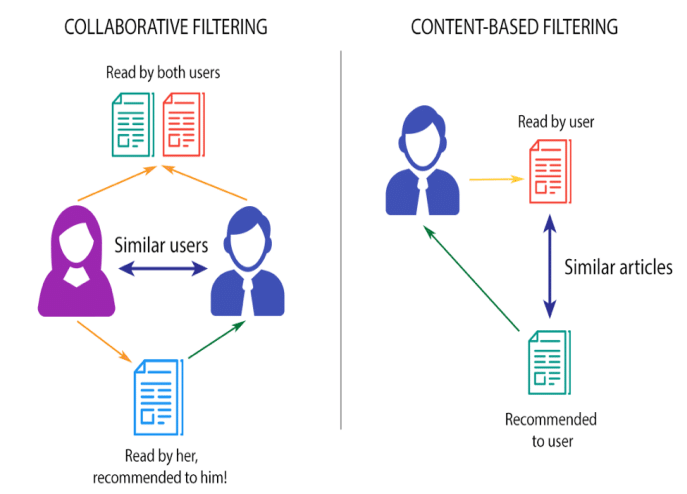
\includegraphics[width=\linewidth]{img/Content-based-filtering-and-Collaborative-filtering-recommendation}
	
\subsubsection{Collaborative Filtering}
\label{sec:Collaborative Filtering}

Het kernidee bij Collaborative Filtering \autocite{Schafera} is om aanbevelingen te maken gebaseerd op de voorkeuren van een andere gebruiker met een gelijkaardig gedrag. Zoals de figuur hierboven aantoont dat als gebruiker 1 en 2 hetzelfde artikel gelezen hebben, gebruiker 2 een artikel als aanbeveling zal krijgen dat gelezen werd door gebruiker 1. 
Hetzelfde idee kan toegepast worden op allerlei interacties van de gebruikers met een website zoals likes, shares, verlanglijstjes, etc.

In de praktijk geeft deze techniek zeer goede resultaten, maar zoals verwacht brengt deze techniek ook enkele problemen met zich mee. Het meest merkwaardige probleem is een zogenaamde cold start, dit komt onder andere voor bij de eerste interactie van een nieuwe gebruiker met een applicatie die aanbevelingen biedt. Het algoritme heeft dan onvoldoende informatie om een correcte en nuttige aanbeveling op te leveren aan de gebruiker. Een andere oorzaak kan zijn dat er een nieuw product wordt toegevoegd aan het systeem, er kan dan nog niet geweten zijn welk type gebruiker hierin geïnteresseerd zou kunnen zijn. 

Een andere factor voor het succes van een Collaborative Filtering algoritme is het aantal gebruikers van een systeem, met andere woorden, hoe meer gebruikers er zijn, hoe correcter de aanbevelingen aan een specifieke gebruiker zal zijn. \autocite{Sarwar2001}. Een gebruiker met ongewone interesses zal logischerwijs in dergelijk klein systeem weinig gelijkaardige gebruikers hebben, en zal dus ook geen optimale aanbevelingen krijgen.


Een groot voordeel van Collaborative Filtering is dat er absoluut geen kennis hoeft te zijn van de toepassing van het systeem, de aanbevelingen worden gegenereerd op basis van het gedrag van de gebruikers en zijn interesses. De producten of hun attributen moeten dus niet gekend zijn om aanbevelingen te kunnen geven, dat maakt het eenvoudiger om een aanbevelingssysteem met de techniek van Collaborative Filtering te implementeren.

\subsubsection{Content Based}
\label{sec:Content Based}

Content Based aanbevelingssystemen \autocite{Lops2011} maken, in tegenstelling tot Collaborative Filtering, wel gebruik van de specifieke producten binnen het systeem en hun attributen. Op basis van deze attributen en de interesse van de gebruiker daarin, wordt per gebruiker een profiel opgezet, elk attribuut krijgt dan een score toegekend, een hogere score betekent grotere interesse. Een attribuut van een product kan dan bijvoorbeeld 'schoenen' of 'PS4 games' zijn, of zelfs een filmgenre.

Een probleem van Content Based is, net zoals bij Collaborative Filtering, het cold start probleem. Als een nieuwe gebruiker het systeem gebruikt, is er voor deze gebruiker nog geen profiel opgesteld en kunnen er ook geen anbevelingen gemaakt worden.

Een ander probleem van Content Based wordt overspecialisatie genoemd, dit treedt op wanneer het systeem eigenlijk té accurate aanbevelingen doet. Het gevolg hiervan is dat slechts enkele producten voldoen aan de verwachtingen van het systeem, waardoor er geen nieuwe aanbevelingen aan de gebruiker naar voor gebracht worden, en de gebruiker enkel producten zal zien die hij reeds bekeken heeft. 

Het andere probleem dat optreedt bij Collaborative Filtering, namelijk dat bij het toevoegen van nieuwe producten niet geweten kan zijn welke gebruikers hierin geïnteresseerd zouden zijn, is niet van toepassing bij Content Based. Het systeem maakt gebruik van de attributen van producten, dus nieuwe producten kunnen meteen belanden in de aanbevelingen van gebruikers die reeds interesse getoond hebben in andere producten met die attributen. Ook het aantal gebruikers binnen een systeem vormt om dezelfde reden geen probleem bij Content Based aanbevelingssystemen. 

Een grote boosdoener bij Content Based kan zijn dat producten slecht gelabeld zijn, en hun attributen onvoldoende passen bij wat het product effectief is. Hierdoor kan het systeem deze producten niet goed vergelijken met andere. Dit is vooral een probleem wanneer de attributen van de producten van verschillende bronnen afkomstig zijn, of manueel slecht opgesteld zijn.

\subsubsection{Hybrides}
\label{sec:Hybrides}

Beide van de voorgenoemde technieken hebben elk hun eigen voor- en nadelen, alsook sterke en zwakke punten. Content Based heeft te kampen met overspecialisatie, maar is wel in staat om nieuwe producten meteen aan te bevelen aan de gebruikers. Collaborative Filtering heeft moeite met het aanbevelen van nieuwe producten en een cold start, maar heeft geen problemen in de aard van overspecialisatie.

De logische redenering is dan natuurlijk om deze twee soorten systemen te gaan combineren, kwestie van het beste van twee werelden te proberen bekomen. Dit worden hybride aanbevelingssystemen \autocite{Cano2017} genoemd.

De manier van het opbouwen van een hybride systeem kan zijn dat beide methoden afzonderlijk worden uitgevoerd, en hun resultaten op het einde samengebundeld worden. Dit is de meest eenvoudige implementatie.

Een andere manier van combineren kan zijn door de informatie binnen een Collaborative Filtering systeem aan te vullen met informatie uit de gebruikersprofielen. Hierdoor wordt de gelijkaardigheid van twee producten bepaald door zowel de inhoud en welke soorten typische gebruikers deze producten bekijken, kopen, leuk vinden, etc.
De informatie van deze gebruikers kan dan bijvoorbeeld leeftijdsgroep, woonplaats, gezinssamenstelling, etc. voorstellen.


\section{Wat is Graph?}
\label{sec:wat is Graph?}

In de context van deze bachelorproef zal er met 'Graph' steeds verwezen worden naar een Graph databank. In dit onderdeel zullen we wat dieper ingaan op wat dit soort databank precies inhoudt om een volledig begrijpen van de precieze werking te verzekeren. 

\subsection{Graph}
\label{sec:Graph}

Graph is de databankstructuur die verder in dit onderzoek gebruikt zal worden. Deze structuur maakt gebruik van een wiskundige graaf om data op te slaan. Een graaf bestaat uit een aantal knopen (genaamd nodes) die al dan niet verbonden zijn. 

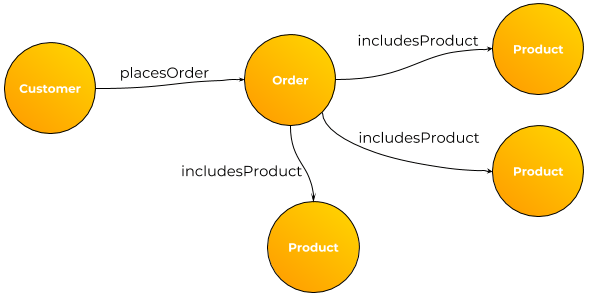
\includegraphics[width=\linewidth]{img/Customer-Order-Example-Graph.png}

Relaties hebben de prioriteit bij een graph databank, dit betekend dat relaties tussen knopen gepersisteerd worden in de databank, en niet enkel tijdelijk berekend voor een enkele query, dit is de reden waarom er geen complexe JOIN query's of foreign keys nodig zijn.

Graph databanken hebben dus een voordeel voor functionaliteiten zoals netwerken, aanbevelingen, etc. maar ook fraudedetectie. 

\subsubsection{Voordelen}
\label{subsec:Voordelen Graph}

Een groot voordeel van de graafstructuur die deze databanken gebruiken is dat deze sneller zijn dan relationele databanken omdat ze op zeer korte tijd naar een bepaalde node kunnen verwijzen, waarbij we bij een relationele databank een JOIN zouden moeten gebruiken. 

Graph databanken zijn ook zeer flexibel in gebruik. Bij het veranderen van een model kan er steeds verder gebouwd worden op het bestaande model, zonder dat hierdoor reeds verwezenlijkte functionaliteiten verloren zou kunnen gaan.
Dit is ook een voordeel bij het opstarten, er moet niet op voorhand grondig gediscussieerd worden over hoe het model er uiteindelijk uit zal moeten zien.

Deze troeven zijn niet te vinden bij traditionele databankstructuren die met tabellen werken, daarbij moet er alvorens het opzetten van de databank al een zekerheid zijn van hoe het model eruit zal zien, want het model zal de mogelijke functionaliteiten bepalen. Als er dan achteraf nog veranderingen nodig zijn, zal heel het model herzien moeten worden.

Nog een belangrijk voordeel van graph databanken is dat hiermee een \textit{Knowledge Graph} kan opgebouwd worden, hier wordt in een verder hoofdstuk van de literatuurstudie dieper op ingegaan.

\subsubsection{Nadelen}
\label{subsec: Nadelen Graph}

Graph databanken hebben niet enkel voordelen, deze zijn vooral afhankelijk van de verwachtingen van de gebruikers en wat zij nodig hebben om hun doeleinden te bereiken. Graph databanken bestaan niet om relationele databanken te vervangen, zij bieden slechts een oplossing voor de beperkingen waar relationele databanken mee kampen.

Graph databanken zijn geen goede keuze wanneer er data moet opgeslagen worden waarbij geen verbanden of connecties zijn tussen deze data, hier blinkt een relationele databank dan weer in uit. 

Hetzelfde geldt voor wanneer de databank slechts als opslag gebruikt zal worden, of er slechts simpele query's nodig zullen zijn die in een relationele databank zonder JOIN statement kunnen gebeuren.Dit is niet zozeer een nadeel, maar benadrukt wel dat graph databanken geen universele \textit{one size fits all} oplossing zijn. Graph kan dit, maar is hiervoor niet geoptimaliseerd.

Een voordeel dat eigenlijk als nadeel kan aanzien worden is dat de data niet consistent hoeft te zijn. Het model dat opgebouwd wordt is niet hetzelfde als een schema bij relationele databanken. Even een kort voorbeeld:

Bij relationele databanken zijn deze objecten gebonden aan een schema van tabellen waar de relaties vooraf gedefinieerd zijn. Hierin wordt dus afgedwongen dat een Persoon werkzaam kan zijn bij een bedrijf, en een persoon een huisdier kan hebben. Het is dus niet mogelijk om een huisdier in te voeren als werkzaam zijnde bij een bedrijf.
Een graph databank zal het toestaan om een relatie van het huisdier als 'werknemer' te leggen naar het bedrijf, aangezien dit soort databank niet gebonden is aan een schema. Dit is natuurlijk niet wenselijk.

De voor- en nadelen van graph databanken worden nog even kort opgesomd in volgende tabel:

\begin{center}
	\begin{tabularx}{\textwidth}{|X|X|}
		\hline
		\textbf{Voordelen} & \textbf{Nadelen}  \\ 
		\hline
		 - Sneller dan relationele databanken bij het queryen met meerdere tabellen & -Gaat slecht om met data waar weinig of geen connecties zijn \\ 
		- Flexibel & - Data is niet gebonden aan een schema \\
		- Makkelijk te begrijpen structuur & - Niet geoptimaliseerd voor simpele query's waar in een relationele databank geen JOIN nodig is \\ 
		- Opbouwen van Knowledge Graph & \\
		\hline
	\end{tabularx}
\end{center}

\subsection{Knowledge Graphs}
\label{sec:Knowledge Graphs}

Google startte in mei 2012 een initiatief genaamd \textit{Knowledge Graph} \autocite{GoogleKnowledgeGraph}. Deze graaf wordt door Google gebruikt om de resultaten van de Google zoekmachine aan te vullen met informatie uit verscheidene bronnen, om zo beknopt aan de gebruikers de meest belangrijke informatie te kunnen tonen zonder dat zij zelf op verschillende resultaten moeten klikken om hun antwoord te vinden. 

De informatie uit deze Knowledge Graph is terug te vinden in een kader rechts van de gewone resultaten, zoals te zien is in volgende figuur. Dit kader werd door Google ook wel het \textit{'Knowledge Panel'} genoemd. 

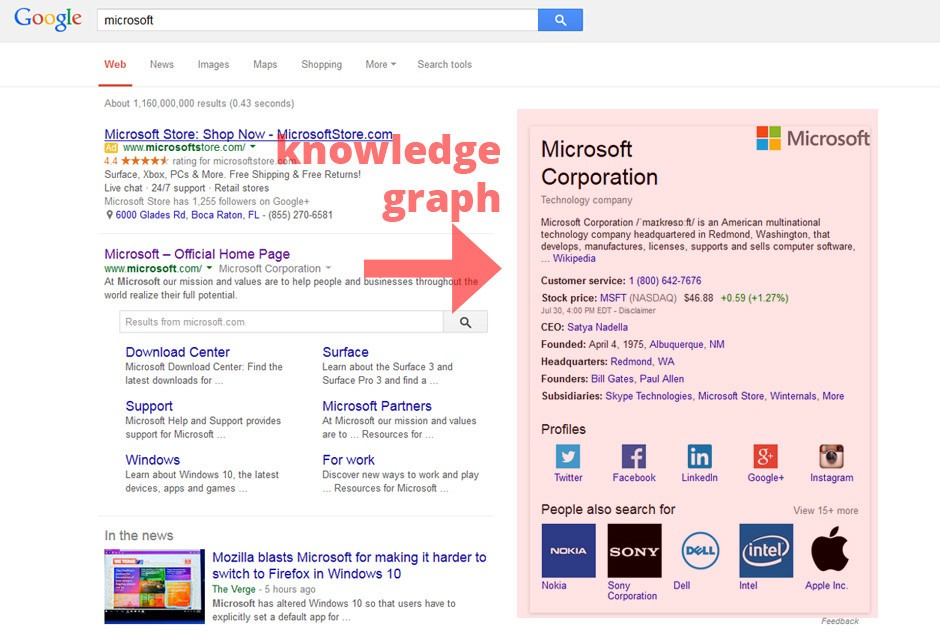
\includegraphics[width=\linewidth]{img/Google_Knowledge_Graph.jpeg}

Sinds de uitvoering van de Google Knowledge Graph is deze term zelf bekend geraakt, en wordt deze algemeen gebruikt voor het representeren van kennis die gebaseerd is op een graaf.

Binnen de informatica worden knowledge graphs ook wel ontologieën genoemd, dit soort graaf houdt eigenlijk een verzameling van onderling gelinkte objecten en feiten bij, die zowel door mensen als computers eenvoudig en ondubbelzinnig te begrijpen zijn.   

Op dezelfde manier dat Google zijn eigen Knowledge Graph gebruikt om haar zoekresultaten te verbeteren, kan er ook een graaf opgesteld worden voor andere toepassingen zoals een webshop. In de context van e-commerce toepassingen kan deze graaf gebruikt worden om relaties tussen producten te ontdekken. 

Aangezien het doorlopen van een graaf zoals eerder besproken zeer snel kan gebeuren, is dit een ideale troef om gepersonaliseerde zoekresultaten te kunnen aanbieden aan gebruikers. \autocite{E-CommerceKnowledgeGraph}

Door middel van een graaf kan geanalyseerd worden welke soorten producten vaak samen gekocht of bekeken worden, alsook ontdekken in welke producten gebruikers van e-commerce toepassingen geïnteresseerd zijn. Op basis hiervan kunnen aanbevelingen berekend en aan de gebruiker getoond worden. 

In de context van aanbevelingssystemen worden knowledge graphs vooral gebruikt om extra kennis toe te voegen aan een graaf met relaties tussen klanten en producten, waardoor er onderling meer connecties kunnen gelegd worden tussen klanten en producten, hierdoor zijn de mogelijkheden voor aanbevelingen plots enorm veel groter.
 
Het cold-start probleem dat eerder bij het puntje aanbevelingssystemen besproken werd, wordt hier ook deels mee opgelost. Als er weinig relaties zijn tussen klant en product, of in het geval van een cold-start zelfs geen, kan de knowledge graph, die kennis heeft over de producten en hoe populair deze zijn, hier een handje bij toesteken om toch succesvol aanbevelingen aan de gebruiker te bieden.

In het onderzoek van \cite{Grad-Gyenge2015} wordt een model voorgesteld waar attributen van bijvoorbeeld een persoon of een film wordt voorgesteld als een extra knoop in een graaf. Zo kunnen films gelinkt worden aan genres, jaar van release, acteurs, etc. en personen kunnen gelinkt worden aan een leeftijd, geslacht, locatie, etc.
Zo kunnen er bogen in de graaf toegevoegd worden die personen met bijvoorbeeld dezelfde interesses en leeftijd groeperen. 

Het is ook een mogelijkheid om gewichten toe te kennen aan deze relaties (bogen), zodat bijvoorbeeld interesse in genres harder doorweegt dan gelijkaardige leeftijd wanneer er een verband gelegd wordt tussen twee personen, op deze manier kunnen de aanbevelingen op maat gegenereerd worden voor andere toepassingen, zoals e-commerce, waar in sommige sectoren leeftijd misschien een belangrijkere relatie is dan regio.

\subsection{Neo4j}
\label{sec:Neo4j}

Er bestaan verschillende platformen voor SQL en relationele databanken, bijvoorbeeld Microsoft SQL Server, MySQL, Oracle, etc.
  
Zo zijn er ook verschillende platformen voor de hierboven beschreven NoSQL databanken, afhankelijk van welk type databank gezocht wordt. Neo4j is een van de meer bekende platformen voor graph databanken, dit platform zal gebruikt worden in dit onderzoek.

Walmart maakt gebruik van Neo4j om de aanbevelingen voor hun klanten op hun online webservices te optimaliseren \autocite{neo4jWalmart2014}. Zij gebruiken dit omdat graph databanken zeer snel over een gebruiker zijn koophistorie kunnen traverseren, en ook direct nieuwe mogelijke interesses kunnen halen uit het gedrag van de gebruiker. Daarmee wordt bedoeld dat er in real-time nieuwe connecties worden gelegd tussen de gebruiker en de producten, en hij de nieuwe aanbevelingen meteen zal zien, en niet enkele dagen of uren later. Er wordt dus historische data gematcht met real-time data, hier blinkt Neo4j in uit. 

Neo4j maakt dus gebruik van wiskundige grafen om data weer te geven samen met hun onderlinge relaties. Een graaf kan gericht of ongericht zijn, ongericht wil zeggen dat er geen richting is waarin de relaties lopen, dus deze zijn onderling uitwisselbaar. 

Een gerichte graaf is dan een graaf waarbij de relaties in een specifieke richting lopen, zoals volgers op Twitter: Persoon A volgt persoon B, maar persoon B volgt niet persoon A. Voor een voorbeeld van hoe een graaf voor Twitter er in simpele vorm uit zou kunnen zien, is zichtbaar in volgende figuur:

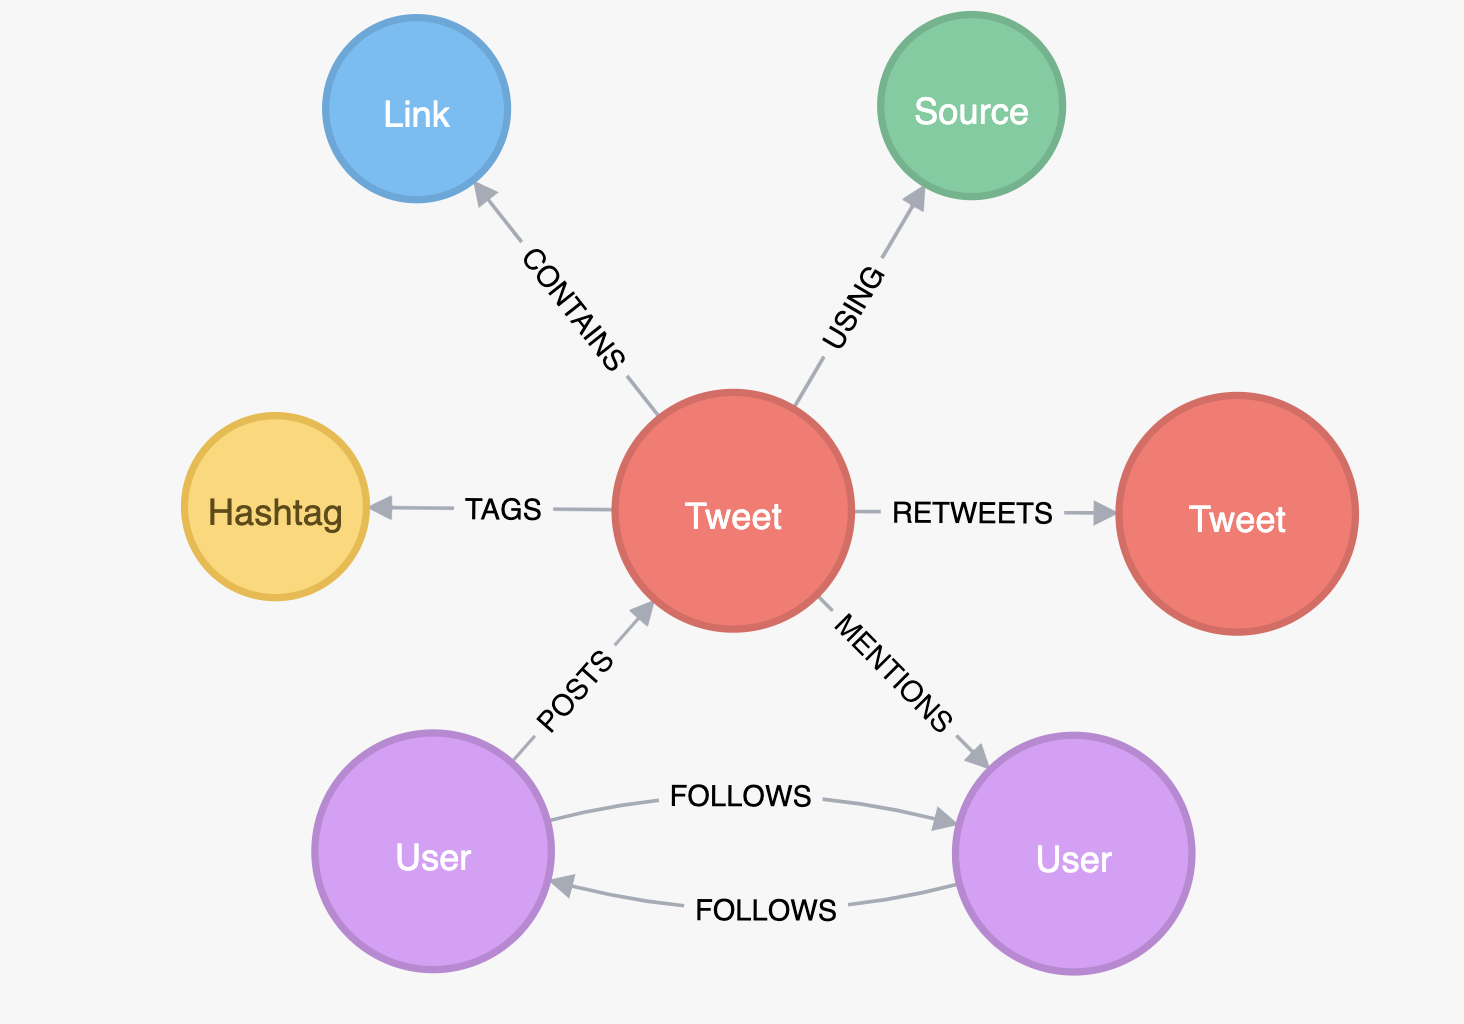
\includegraphics[width=\linewidth]{img/twitter_graph}

\subsubsection{Performantie}
\label{subsubsec:Performantie}

In in hoofdstuk één van het boek 'Neo4j in Action' \autocite{Vukotic2014} wordt een onderzoek gedaan naar de snelheid van het uitvoeren van bepaalde query's zoals 'zoek vrienden van vrienden' op een dataset. De resultaten hiervan wijzen erop dat graph databanken beduidend sneller zijn in het traverseren van een graaf, bijvoorbeeld voor het zoeken op een bepaalde diepte vanaf een startpunt.

Het experiment bestaat eruit 'vrienden van vrienden' op te halen uit een databank, dit in zowel Neo4j als MySQL. De databank bestaat voor beide platformen uit 1 000 000 gebruikers, \textit{Execution Time} wordt uitgedrukt in seconden per 1000 gebruikers.

In Tabel 2.1 worden de resultaten van dit experiment samengevat. De \textit{Depht} slaat hier op hoeveel vrienden een persoon van een andere persoon verwijderd zal zijn, voor een diepte drie is dit dus 'vrienden van vrienden van vrienden'.

	\begin{table}
		\centering
		\begin{tabular}{|l|l|l|}
			\hline
			Depth & Execution Time - MySQL                                & Execution Time - Neo4j \\ \hline
			2     & 0.016                                                 & 0.010                  \\ \hline
			3     &  30.267 & 0.168                  \\ \hline
			4     & 1,543.505                                             & 1.359                  \\ \hline
			5     & Not Finished in 1 Hour                                & 2.132                  \\ \hline
		\end{tabular}
	\caption{\label{tab:Neo4j - MySql Comparison} Source: https://neo4j.com/news/how-much-faster-is-a-graph-database-really/}
	\end{table}


Uit deze resultaten wordt al snel duidelijk dat Neo4j drastisch beter presteert bij het zoeken binnen netwerken van entiteiten waar veel connecties tussen voorkomen, wat nogmaals bevestigd dat voor dit soort use-cases, graph databanken de beste keuze zijn.



\section{Wat is ElasticSearch?}
\label{sec:wat is ElasticSearch?}

Elasticsearch op zichzelf is eigenlijk een zoekmachine die data kan analyseren, of dit nu nummers, tekst, gestructureerd of ongestructureerd is. 

Elasticsearch is een component van de Elastic stack, ook wel ELK-Stack genoemd. Dit staat voor Elasticsearch, Logstash en Kibana. Logstash wordt gebruikt om data te verwerken uit meerdere bronnen en te versturen naar Elasticsearch. Kibana is een tool om de gebruikers een visueel beeld te geven van de data in de vorm van grafieken of tabellen.

Data wordt in Elasticsearch opgeslagen als een document in JSON-formaat in een index. Aangezien dit een zoekmachine is, is Elasticsearch dus gespecialiseerd in het zoeken van data, bijvoorbeeld een query om alle producten op te halen waar het woord 'switch' in voorkomt zal zeer snel resultaten opleveren.  

Elasticsearch ondersteunt ook meerdere methodes voor het zoeken, eentje ervan is zoals hierboven beschreven het zoeken op een stukje tekst, waarbij alle documenten geretourneerd worden waar de tekst in een van de velden voorkomt, dit wordt tekst-gebaseerd zoeken genoemd.  Hieronder enkele voorbeelden van zoekmethodes:  

De zoekmethode die hier als voorbeeld genomen werd maakt gebruik van de parameter \textit{query\textunderscore string}. Als een van de velden van een document overeenkomt met de ingevoerde tekst, zal dit document in de lijst van resultaten terechtkomen.

\begin{lstlisting}[caption={Tekst-gebaseerd zoeken: Query om een simpele zoekopdracht uit te voeren met de term 'deodorant'}]
{
	"query" : 
	{
		"query_string": 
		{
			"query": "deodorant"
		}
	}
}
\end{lstlisting}

Er kan ook op specifieke termen gezocht worden via \textit{term}. Daarbij kan dan gespecificeerd worden welk veld moet overeenkomen met de ingevoerde tekst. 
Indien men wil zoeken op meerdere termen, kan terms vervangen worden door de parameter \textit{terms}, en zal er een array mee moeten gegeven worden als input in plaats van 'Audio' 

\begin{lstlisting}[caption={Tekst-gebaseerd zoeken: Query om een simpele zoekopdracht uit te voeren waar de categorie van het product overeen komt met 'Audio' }]
{
	"query" : 
	{
		"term": 
		{
			"category": "Audio"
		}
	}
}
\end{lstlisting}

Een andere manier om te zoeken op basis van tekst is \textit{match}. Hierbij worden alle woorden van alle velden van een document bekeken, en wordt er een score toegekend voor elke keer dit woord in het document voorkomt, op deze manier zullen resultaten waarbij dit woord het vaakst voorkomt, bovenaan in de lijst van resultaten terechtkomen. 

\begin{lstlisting}[caption={Tekst-gebaseerd zoeken: Query die de resultaten sorteert op basis van hoe vaak het woord 'accepted' voorkomt in het veld 'message' van een document }]
{
	"query" : 
	{
		"match": 
		{
			"message": "accepted"
		}
	}
}
\end{lstlisting}

Als men wil zoeken binnen een bepaalde prijsklasse, bijvoorbeeld tussen 30 en 50 euro, kan dit met de parameter \textit{range}, bijvoorbeeld met volgende query:

\begin{lstlisting}[caption={Bereik zoeken: Een query om alle documenten op te halen waarbij het veld 'price' tussen 30 en 50 ligt}]
{
	"query" : 
	{
		"range": 
		{
			"price": {
				"gte": 30,
				"lte": 50
			}
		}
	}
}
\end{lstlisting}


Het is ook mogelijk om query's te combineren, dit kan verwezenlijkt worden door het gebruik van een \textit{bool query}. De parameters die hieronder gebruikt kunnen worden zijn:

\begin{itemize}
	\setlength\itemsep{1em}
	\item \textit{``must``} : De meegegeven waarde moet in het document voorkomen en de score van deze query zal meetellen voor de totale score. Dit is een strikte voorwaarde, als hier niet aan voldaan wordt zal het document niet opgenomen worden in de resultaten.	
	\item \textit{``filter``} : De meegegeven waarde moet in het document voorkomen. De score van deze query zal niet meetellen voor de totale score. Alle documenten die niet aan de voorwaarden van de filter voldoen, zullen net zoals bij 'must' niet opgenomen worden in de resultaten.	
	\item \textit{``should``} : Als de gegeven waarde voorkomt in het document, zal de score van het document verhoogd worden, maar dit is geen strikte voorwaarde. De parameter \textit{``minimum\textunderscore should\textunderscore match``} geeft aan aan hoeveel voorwaarden voldaan moet worden om het document op de nemen in de resultaten. De \textit{``boost``} parameter laat toe bepaalde overeenkomsten een hogere score te laten genereren.
	\item \textit{``must\textunderscore not``} : Het omgekeerde van 'must'. De meegegeven waarde mag niet voorkomen in het document. Net zoals bij 'filter' zal de score voor deze query niet meetellen. 
\end{itemize}

\begin{lstlisting}[caption={Combineren: Voorbeeld van een 'bool' query}]
{
	"query" : 
	{
		"bool": 
		{
			"must": {
				"term" : { "name" : "Kim" }
			},
			"must_not": {
				"term": { "lastname" : "Johnson" }
			},
			"filter": {
				"term": { "gender" : "female" }
			},
			"should" : [
				{
					"range" : {
						"age" : { "gte" : 20, "lte" : 30 }
					}
				},
				{
					"range" : {
						"height" : { "gte" : 150, "lte" : 170 } ,
						"boost" : 3
					}
				},
				{
					"term" : { "country" : "Belgium" }
				},
			],
			"minimum_should_match": 2
		}
	}
}
\end{lstlisting}
 
Bovenstaande query zal alle documenten retourneren waar: 
\begin{itemize}
	\setlength\itemsep{.3em}
	\item De voornaam 'Kim' is
	\item De achternaam NIET 'Johnson' is
	\item Het geslacht 'female' is.
\end{itemize}

En er aan minstens twee van deze drie voorwaarden voldaan wordt: 
\begin{itemize}
	\setlength\itemsep{.3em}
	\item De leeftijd tussen 20 en 30 jaar is
	\item De lengte tussen 150 en 170 is
	\item Het land 'België' is.
\end{itemize}



In Elasticsearch is het dus mogelijk gewichten toe te kennen aan de resultaten van een zoekopdracht, zo kunnen meer relevante resultaten hoger in de lijst staan, dit is een belangrijke factor in dit onderzoek, namelijk of deze technologie gebruikt kan worden in E-Commerce toepassingen.

Een alternatieve en meer uitgebreide manier om scores toe te kennen aan resultaten is via een \textit{``function\_score``}. Het bovenste deel van deze query (\textit{``query``}) zal bepalen welke documenten opgenomen moeten worden, en het onderste deel ( \textit{``functions``}) zal een lijst van functies vormen. 

Aan de hand van deze functies zal een score voor een resultaat worden berekend. Aan elk van deze functies kan een gewicht (\textit{``weight``}) worden toegekend om bepaalde overeenkomsten meer te laten doorwegen dan andere en deze dus een hogere score toe te kennen.

Er komen nog twee extra parameters kijken bij deze functies, namelijk \textit{``score\_mode``} en \textit{``boost\_mode``}. Elk document dat wordt opgehaald zal een score toegewezen krijgen. 

De parameter score\_mode bepaalt hoe de scores  van deze functies gecombineerd worden. Mogelijke opties hiervoor zijn \textit{``multiply``}, \textit{``sum``}, \textit{``avg``}, \textit{``first``}, \textit{``max``}, en \textit{``min``}

De parameter boost\_mode bepaalt hoe de score van de query en de functies gecombineerd moet worden. Mogelijke opties hiervoor zijn: \textit{``multiply``}, \textit{``replace``}, \textit{``sum``}, \textit{``avg``}, \textit{``max``}, en \textit{``min``}.

De meeste opties verklaren zichzelf, \textit{``replace``} zal de score die toegekend werd aan het document bij het ophalen ( \textit{``query``}) overschrijven door de score die berekend werd door de functies. 

Hieronder een voorbeeld van een function\_score query waar alle documenten opgehaald worden, daarna zal er een score van 4 toegekend worden aan de documenten indien 'name' overeenkomt met 'Kim', en een score van 2 indien 'age' overeenkomt met '23'.

De scores van deze functies zullen worden opgeteld, en het resultaat hiervan zal de score die toegekend werd aan het resultaat bij het ophalen van het document overschrijven. 

\begin{lstlisting}[caption={Scoring: voorbeeld van een function\_score query}]
{
	"query" : {
		"function_score" : {
			"query" : { "match_all" : {} },
			"boost" : 2,
			"functions" : [
				{
					"filter" : { "match" : { "name" : "Kim" } },
					"weight": 4
				},
				{
				"filter" : { "match" : { "age" : 23 } },
				"weight": 2
				}
			],
			"score_mode" : "sum",
			"boost_mode" : "replace"
		}
	}
}
\end{lstlisting}

De \textit{``script\_score``} functie laat toe om een score voor een document te berekenen aan de hand een van de waarden van de velden in het document.

Onderstaande query zal alle documenten ophalen waarbij het veld 'naam' overeenkomt met 'Kim', en zal een score berekenen op basis van de lengte. In dit geval (300 - lengte) zal een lagere waarde voor dit veld resulteren in een kleinere score.

\begin{lstlisting}[caption={Scoring: voorbeeld van een script\_score query}]
{
	"query" : {
		"script_score" : {
			"query" : {
				"match" : { "name" : "Sasha" }
			},
			"script": {
				"
				height = doc['height'].value;
				return 300 - height;
				"
			}
		}
	}
}
\end{lstlisting}

Decay functies kunnen gebruikt worden om de score van een document aan te passen naar gelang een opgegeven veld afwijkt van een bepaalde waarde. Dit is gelijkaardig aan de 'range' query, waar met met intervallen zou kunnen werken, maar loopt geleidelijk mee naargelang de afstand tussen de waarde van het veld en de opgegeven waarde groter wordt. 
\newline

Er zijn drie mogelijke decay functies, namelijk \textit{``linear``}, \textit{``exp``}, en \textit{``gauss``}. De velden die hierbij horen zijn:

\begin{itemize}
	\item \textit{``origin``} : Het startpunt voor het berekenen van de afstand. De waarde hiervan moet numeriek, een datum of een geo-punt zijn.
	\item \textit{``scale``} : Het verschil dat nodig is om de score te doen afnemen met de waarde aangegeven door de decay.
	\item \textit{``offset``} (Optioneel):  Als deze waarde gedefinieerd wordt, zal de decay functie enkel berekend worden als de afstand groter is dan deze waarde. Default is 0.
	\item \textit{``decay``} (Optioneel): Geeft aan met welke waarde de score van een document moet afnemen. Default is 0.5
\end{itemize}


\begin{lstlisting}[caption={Decay: voorbeeld van een decay functie}]
{
	"query" : {
		"function_score" : {
			"exp" : {
				"date" : {
					"origin": "2013-09-17",
					"scale" : "10d",
					"offset" : "5d",
					"decay" : 0.5				}
			}
		}
	}
}
\end{lstlisting}

De bovenstaande query zal de score van een document laten afnemen met 0.5 naar gelang de waarde van het veld 'datum' verder ligt van de opgegeven waarde (2013-09-17). De waarde zal niet afnemen indien deze binnen de 5 dagen verwijderd ligt van de opgegeven waarde.

 In het artikel van \autocite{Vavliakis2019} wordt beweerd dat het systeem dat zij implementeerden op een performante manier de gewenste resultaten gaf, alsook dat dit een oplossing kan zijn voor real-time zoekopdrachten in commerciële toepassingen. Dit sluit dus al uit dat Elasticsearch geen oplossing zou kunnen bieden voor onze onderzoeksvraag.
 
\section{Filter Bubble}
\label{sec:Filter Bubble}

Een filter bubble, ook wel informatieluchtbel genaamd, is een gevolg van het personaliseren van zoekopdrachten. Personalisatie is het proberen bepalen welke zaken een gebruiker zou willen zien, aan de hand van een algoritme. 

Een filter bubble betekent dat door deze personalisatie, een bijvoorbeeld geen producten zal zien die hem niet interesseren, in dit geval is dat een voordeel. Als we kijken in de context van controversiële onderwerpen, zorgt deze bubbel ervoor dat de gebruiker eigenlijk geen informatie zal zien die niet bij zijn standpunt past, de gebruikers worden dus afgesloten in luchtbel bestaande uit enkel hun visie of standpunt.  \autocite{Pariser2011}

Pariser geeft als voorbeeld in zijn boek een scenario waar een gebruiker de zoekterm ``BP``invoerde, en resultaten kreeg in verband met investeringsnieuws over British Petroleum. Een tweede gebruiker gaf dezelfde zoekterm in en kreeg informatie over Deepwater Horizon als resultaat. Dit is dus een merkwaardig verschil.

Parser beweert dat het effect van de filter bubble negatieve gevolgen kan hebben voor de manier waarop mensen hun mening vormen, dit aangezien zij geen argumenten te zien krijgen die hun mening tegenspreken.


De relevantie van dit fenomeen voor dit onderzoek valt op het feit dat bij de Content Based algoritmen die eerder besproken werden, we met een gelijkaardig probleem te maken hadden. Bij deze aanbevelingssystemen kan er overspecialisatie optreden, waardoor de gebruiker enkel producten aanbevolen krijgt die reeds gezien zijn, of té gelijkaardig zijn, en er dus geen nieuwe verrassende producten aangeboden worden.

\section{GDPR}
\label{sec:GDPR}



%%=============================================================================
%% Methodologie
%%=============================================================================


\chapter{\IfLanguageName{dutch}{Methodologie}{Methodology}}
\label{ch:methodologie}


Rekeninghoudend met de bevindingen uit de literatuurstudie, zal hier verder besproken worden hoe we een systeem gaan opstellen dat gepaste aanbevelingen kan maken. Gezien we twee verschillende werkwijzen en technologieën zullen vergelijken, zal voor beide systemen een werkwijze voorgesteld worden. Deze werkwijze zal ook in dit hoofdstuk verder uitgewerkt worden.

\section{Uitwerking ElasticSearch}
\label{sec:Uitwerking ElasticSearch}

Voor de uitwerking van Elasticsearch wordt een instantie opgezet waarmee we zullen communiceren, op deze instantie draait Elasticsearch. 

In Elasticsearch worden items opgeslagen als een document met enkele waarden, typisch aan een product. In dit onderzoek zijn deze waarden; 'naam', 'merk', 'categorieën', en 'prijs'. 

\subsection{Producten}
\label{sec:Producten}
Voor het aanmaken van de product data zullen enkele query's uitgevoerd worden die er als volgt uitzien:

\newpage
\begin{lstlisting}[caption={Query om één enkel product aan te maken},captionpos=b]
POST http://35.233.112.106:9200/products/product/1 
{ 
 "name": "Logitech G930",
 "brand": "Logitech",
 "categories": ["Headset", "Wireless headset", "Headphones"],
 "price": "190.00"
}
\end{lstlisting}

Op deze manier worden enkele producten in de databank gezet, met enkele verwante velden zoals gelijkaardige categorieën, zodat we hiermee aanbevelingen kunnen maken. Deze verzameling van producten wordt een index genoemd.

Vervolgens kunnen we een zoekterm ingeven via volgende query, deze zal alle resultaten weergeven waarvan een van de velden voldoet aan de meegegeven waarde, namelijk "deodorant". 

\begin{lstlisting}[caption={Query om één enkel product op te halen},captionpos=b]
GET http://35.233.112.106:9200/products/product/1 
{
 "query" : {
  "query_string": {
   "query": "deodorant"
  }
 }
}
\end{lstlisting}

\subsection{Gebruikers}

Er zullen enkele vooraf gedefinieerde gebruikers opgesteld worden, waarmee bepaald zal worden of de zoekresultaten aan de verwachtingen voldoen. Een voorbeeld van een gebruiker is te zien in volgende query:
\begin{lstlisting}[caption={Query om één enkele gebruiker aan te maken}]
POST http://35.233.112.106:9200/users/user/1
{
	"name": "Louise",
	"age": "21",
	"address": {
		"city": "Aalst",
		"street": "Molendries 4",
		"province": "Oost-Vlaanderen"
	},
	"categories": ["Electronics, Apple"],
	"searches": ["iphone", "deodorant", "uncommon product"],
	"brands": ["Nivea", "Apple"]
}
\end{lstlisting}

Bij deze gebruiker kunnen we bijvoorbeeld verwachten dat als deze 'deodorant' opzoekt, zij die van het merk Nivea bovenaan de resultaten zal zien. 

Een voorbeeld van zo'n zoekopdracht, waarbij sommige velden ingevuld zijn op basis van onze persoon van de query hierboven, gaat als volgt:

\begin{lstlisting}[caption={Query om een zoekopdracht met term 'Deodorant' uit te voeren, met filters en een score op basis van informatie van een gebruiker}]
POST http://35.233.112.106:9200/products/_search
{
  "query": {
    "function_score": {
      "query": {
        "query_string": {
          "query": "Deodorant"
        }
      },
      "functions": [
        { "filter" : 
          { "terms" : 
            { "brand" : ["Niveau", "Apple"]  } 
          },
          "weight": 3
        },
        { "filter" : 
          { "terms" : 
            { "categories" : ["Electronics", "Apple"] }
          },
          "weight": 2
        },
        { "filter" : 
          { "terms" : 
            { "searches" : ["iphone", "deodorant", "uncommon product"] } 
          },
          "weight": 1
        }
      ],
      "score_mode": "sum",
      "boost_mode": "replace"
      }
   }
}
\end{lstlisting}

In het bovenste deel van de query, waar de \textit{query\textunderscore string} wordt aangeduid. Deze string zou dan overeenkomen met wat een gebruiker zou invoeren in een zoekbalk op een website.

In de realiteit zal de informatie over 'brand', 'categories', en 'searches' opgehaald worden uit het model van de persoon in kwestie.

In deze query wordt een score toegekend aan de resultaten die voldoen aan bovenstaande verwachting, namelijk dat het woord 'deodorant' terug te vinden moet zijn in een van de velden van het product (naam, merk, categorie)

\newpage
Die score wordt toegekend op basis van de informatie over een persoon, hieruit verstaan we dat dit gaat over de merken die deze persoon reeds gekocht heeft, in welke categorieën deze persoon reeds gekocht heeft, en een historiek van zoekopdrachten. Deze hebben elk een gewicht toegekend gekregen, respectievelijk drie, twee en één. 

In de query zijn drie filters te zien die de score van een resultaat zullen beïnvloeden. Bij elk van deze filters wordt het score vermenigvuldigd met het gewicht. \textit{score\textunderscore mode : sum} zorgt ervoor dat de resultaten van de scores opgeteld worden.

\textit{boost\textunderscore mode : replace} zorgt ervoor dat de score die verkregen wordt bij het gelijkaardig zijn aan de zoekterm vervangen wordt door de nieuw berekende score van de functies.

Deze query is een vorm van collaborative filtering, toegepast op zichzelf. De query zal dus gaan zoeken naar hoe verwant een resultaat is aan een persoon, op basis van enkele variabelen, en zal deze een hogere score toekennen afhankelijk van hoe relevant het product is voor een gebruiker. Resultaten met een hogere score zullen dus bijgevolg ook hoger in de lijst van resultaten komen te staan.

\subsection{Graph API Plug-in}
\label{sec:Graph API Plug-in}

Elasticsearch biedt ook een plug-in aan die de functionaliteiten van een graph database voorziet. Met deze plug-in bekomen we dus eigenlijk een Knowledge Graph zoals eerder in de literatuurstudie vermeld werd. 

Deze plug-in laat toe om connecties te vinden tussen objecten in de databank, en wordt geadverteerd als ook bruikbaar te zijn voor aanbevelingen.

Jammer genoeg is deze plug-in enkel beschikbaar wanneer we beschikken over een Platinum of Enterprise licentie. Door deze vereiste valt deze functionaliteit dus buiten de scope van het onderzoek. 

\begin{figure} [ht]
	\centering
	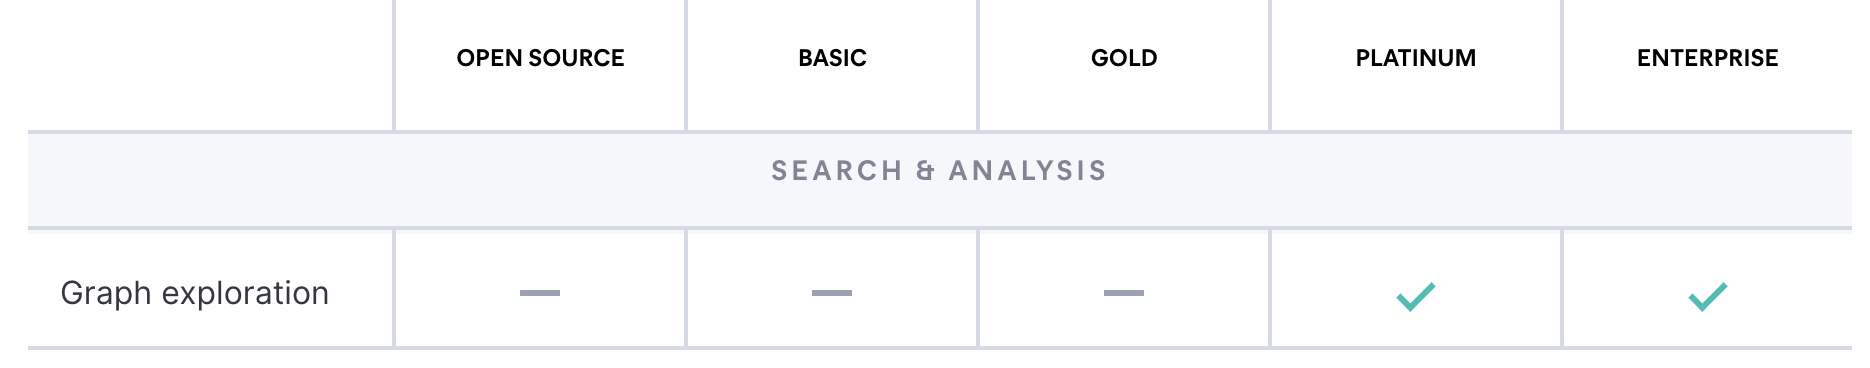
\includegraphics[width=0.95\textwidth]{img/elastic-license}
	\caption{Overzicht van de beschikbaarheid van de Graph plugin voor de Elastic licenties}
	\floatfoot{Source: https://www.elastic.co/subscriptions}
	\label{fig:elastic licenties overzicht graph}
\end{figure}

\newpage
\section{Uitwerking Neo4j}
\label{sec:UItwerking Neo4j}

Voor dit systeem wordt er een model opgesteld in een Graph databank, de gekozen technologie hiervoor is Neo4j. Op deze graaf kunnen dan zoekalgoritmen uitgevoerd worden, om zo tot correcte aanbevelingen te komen. In dit hoofdstuk zal verder uitgewerkt worden hoe dit precies in elkaar zit.

\subsection{Model}
\label{sec:Model}
Relaties tussen producten en klanten zullen als volgt worden opgeslagen in deze Graph databank:

Er zijn 2 soorten nodes, dit zijn de knopen van een graaf, namelijk 'Gebruiker' en 'Product'. De relaties, aangeduid door lijnen tussen de knopen, zullen dan voorstellen wat de interactie van een gebruiker met een product is. Dit kan 'LIKES', 'BOUGHT', of 'LIVES\_TOGETHER' zijn. 'LIVES\_TOGETHER' zal dan aanduiden of 2 gebruikers familie of samenwonend zijn. 

De attributen van een Product zijn als volgt:
\begin{itemize}
	\item Product ID
	\item Name
	\item Brand
\end{itemize}

De attributen voor een Gebruiker zijn als volgt:
\begin{itemize}
	\item Name
	\item Address
\end{itemize}

De verschillende soorten relaties zijn als volgt:
\begin{itemize}
	\item 'BOUGHT' -> Gebruiker heeft Product gekocht
	\item 'LIKES' -> Gebruiker heeft Product leuk gevonden
	\item 'LIVES\_TOGETHER' -> Gebruiker 1 heeft hetzelfde adres als Gebruiker 2
\end{itemize}

Volgende query wordt gebruikt om de product- en klant nodes aan te maken, dit is uiteraard een verkorte versie:

\begin{lstlisting}[caption={Neo4j query voor het aanmaken van producten en klanten}]
CREATE 
(shauni:Customer {name: 'Shauni', address: 'Exterkenstraat 14'}),
(lynn:Customer {name: 'Lynn', address: 'Exterkenstraat 14'}),
(angelo:Customer {name: 'Angelo', address: 'Arbeidstraat 14'}), 
...
(prod1:Product{id: '1', name:'Hairbrush', brand:'Syoss'}), 
(prod2:Product{id: '2', name:'Instant Chocolate Milk', brand:'Nesquick'}), 
(prod3:Product{id: '3', name:'Toilet Paper', brand: 'Boni'}), 
...
\end{lstlisting}

Om een relatie aan te maken tussen een product en een gebruiker zal volgende query gebruikt worden. Deze zal dus uitgevoerd worden elke keer een gebruiker een actie uitvoert met een product.
Aangezien een product leuk vinden en een product kopen niet aanzien worden als evenwaardig, zullen er gewichten toegekend worden aan de interacties tussen gebruikers en producten.  Dat kan door middel van volgende query:

\begin{lstlisting}[caption={Neo4j query voor het aanmaken van een relatie tussen een product en een klant}]
	MATCH (c:Customer),(p:Product) 
	WHERE c.name = 'Shauni' AND p.id=3 
	CREATE (c)-[r:BOUGHT]->(p) 
	SET r.score = 3
\end{lstlisting}

Een product leuk vinden krijgt een score 2 toegekend, en een product kopen zal de score 3 krijgen, om de relatie 'LIKES' aan te maken zal in bovenstaande query de relatie 'BOUGHT' en de score moeten aangepast worden.

Om de relatie van Gebruikers die op eenzelfde adres wonen aan te maken, gebruiken we volgende query: 

\begin{lstlisting}[caption={Neo4j query voor het aanmaken van een relatie tussen een twee klanten.}]
	MATCH (a:Customer), (b:Customer) 
	WHERE EXISTS (a.address) AND EXISTS (b.address) AND a.address=b.address AND id(a)<id(b) 
	CREATE (a)-[:LIVES\_TOGETHER]->(b); 
\end{lstlisting}

De uiteindelijke graaf die voor dit zeer klein voorbeeld opgebouwd werd, zal al snel een beter inzicht geven in hoe deze data aan elkaar vast hangt. Dit is ook een van de troeven van Neo4j, het voorstellen van duidelijke visuele beelden die het eenvoudig maken om te begrijpen wat er zich op de achtergrond afspeelt. De graaf is te zien in Figuur \ref{fig:neo4jfullgraph}
\newpage

\begin{figure} [h!]
	\centering
	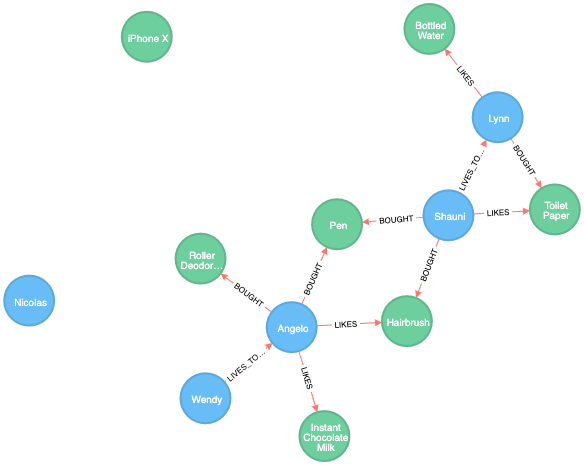
\includegraphics[width=0.95\textwidth]{img/full_graph_result}
	\caption{Overzicht van de ingevoerde data in een Neo4j graaf}
	\label{fig:neo4jfullgraph}
\end{figure}


\subsection{Ophalen van data}
\label{sec:Neo4j Ophalen van data}

Voor deze uitwerking werden enkele query's opgesteld die op basis van de relaties producten retourneren die zouden kunnen dienen als aanbevelingen.

Zo kan er bijvoorbeeld een lijst van producten gegenereerd worden die leuk gevonden of gekocht werden door de familieleden van een bepaalde gebruiker, dit gebeurt op basis van de relatie LIVES\_TOGETHER.

\begin{lstlisting}[caption={Neo4j query die alle likes en aankopen van de familie van een bepaalde gebruiker c1 weergeeft}]
MATCH (c1: Customer)
WHERE c1.name = 'Shauni'
MATCH (c1) - [:LIVES_TOGETHER] -> (c2 : Customer) - [:BOUGHT] -> (p:Product)
RETURN p as Product
UNION
MATCH (c1) - [:LIVES_TOGETHER] -> (c2) - [:LIKES] -> (p:Product)
RETURN p as Product
\end{lstlisting}

Ook van belang is het ophalen van producten die gebruikers kopen waar een gebruiker \textit{c1} gemeenschappelijke aankopen mee heeft. Dit kan via volgende query:

\begin{lstlisting}[caption={Neo4j query die de aankopen van gebruikers weergeeft waar een gebruiker c1 gemeenschappelijke aankopen mee heeft}]
MATCH (c1: Customer)
WHERE c1.name = 'Shauni'
MATCH(c1) - [:BOUGHT] -> (p1 : Product) <- [:BOUGHT] - (c2: Customer) - [:BOUGHT] -> (p2: Product)
RETURN p2
\end{lstlisting}

Om ditzelfde te bereiken maar dan inclusief de likes van deze gebruikers waar een gebruiker \textit{c1} gemeenschappelijke aankopen mee heeft, kan volgende query gebruikt worden: 

\begin{lstlisting}[caption={Neo4j query die de aankopen en likes van gebruikers weergeeft waar een gebruiker c1 gemeenschappelijke aankopen mee heeft}]
MATCH (c1) - [:BOUGHT] -> (p1 : Product) <- [:BOUGHT] - (c2: Customer) - [:BOUGHT] -> (p2: Product)
RETURN p2 as Product
UNION ALL
MATCH (c1) - [:BOUGHT] -> (p1) <- [:BOUGHT] -(c2) - [:LIKES] -> (p2) 
WHERE id(c1)<id(c2)
RETURN p2 as Product
\end{lstlisting}


\subsection{Search}
\label{subsec: Search Neo4j}

Binnen neo4j is het ook mogelijk om zoekopdrachten uit te voeren op basis van een tekstveld. Hiervoor moet op voorhand een index aangemaakt worden waarin beschreven staat welke attributen van welke types van nodes gebruikt mogen worden om de ingevoerde tekst mee te vergelijken.

\begin{lstlisting}[caption={Een index creëren binnen Neo4j om zoekopdrachten op basis van tekst uit te voeren}]
CALL db.index.fulltext.createNodeIndex("namesAndBrands",["Product"],["name", "brand"])
\end{lstlisting}

In dit voorbeeld gebruiken we de attributen \textit{name} en \textit{brand} van het nodetype \textit{Product}, en nemen we als zoekterm ``deodorant``.  Op deze manier kan er dus eenvoudig gekozen worden op welke velden van de objecten er moet vergeleken worden.



\begin{lstlisting}[caption={Een zoekopdracht uitvoeren op basis van tekst}]
CALL db.index.fulltext.queryNodes("namesAndCategories", "deodorant") YIELD node, score
RETURN node.name, node.category, score
\end{lstlisting}

Er zal een lijst geretourneerd worden met de attributen (node.name), en een score die door het algoritme werd toegekend die aantoont hoe sterk het resultaat gelijkend is aan de ingevoerde tekst.

\subsection{PageRank}
\label{subsec:PageRank}

Voor het vinden van resultaten die belang hebben voor de gebruiker, wordt het PageRank algoritme gebruikt. Dit algoritme berekent de belangrijkheid van een knoop op basis van zijn buren. Hoe meer connecties er naartoe, hoe sterker het resultaat. Op deze manier worden populaire resultaten hoger gerangschikt.

Om via dit algoritme aanbevelingen te verkrijgen, moet er eerst een nieuwe graaf worden opgesteld waar enkel de informatie in zit die nodig is voor de berekening, dit gebeurt via volgende query, waarin de interacties 'BOUGHT' en 'LIKES' opgenomen worden, samen met hun gewicht (score).

\begin{lstlisting}[caption={Een genoemde graaf creëren om graafalgoritmen op uit te voeren}]
CALL gds.graph.create.cypher(
	'boughtGraph',
	'MATCH (p:Product) RETURN id(p) AS id',
	'MATCH (p2:Product)<-[r:BOUGHT]-(c:Customer)-[:BOUGHT|LIKES]->(p3:Product)
	RETURN
		id(p2) AS source,
		id(p3) AS target,
		r.score AS score',
		{
			readConcurrency: 4
		}
)
\end{lstlisting}

Vervolgens kunnen we het PageRank algoritme uitvoeren op deze graaf, die een lijst van productnamen zal weergeven met daarnaast een score.

\begin{lstlisting}[caption={PageRank algoritme uitvoeren}]
CALL gds.pageRank.stream('boughtGraph', { maxIterations: 3, dampingFactor: 0.85 })
YIELD nodeId, score
RETURN gds.util.asNode(nodeId).name AS name, score
ORDER BY score DESC, name ASC
\end{lstlisting}

Het resultaat van dit algoritme (Figuur \ref{fig:simplePageRankResult}) toont ons dat ``Wireless Mouse`` de belangrijkste knoop is in deze graaf, met andere woorden dat als er door de graaf gelopen wordt, deze knoop de grootste kans heeft om bereikt te worden. 

\begin{figure} [ht]
	\centering
	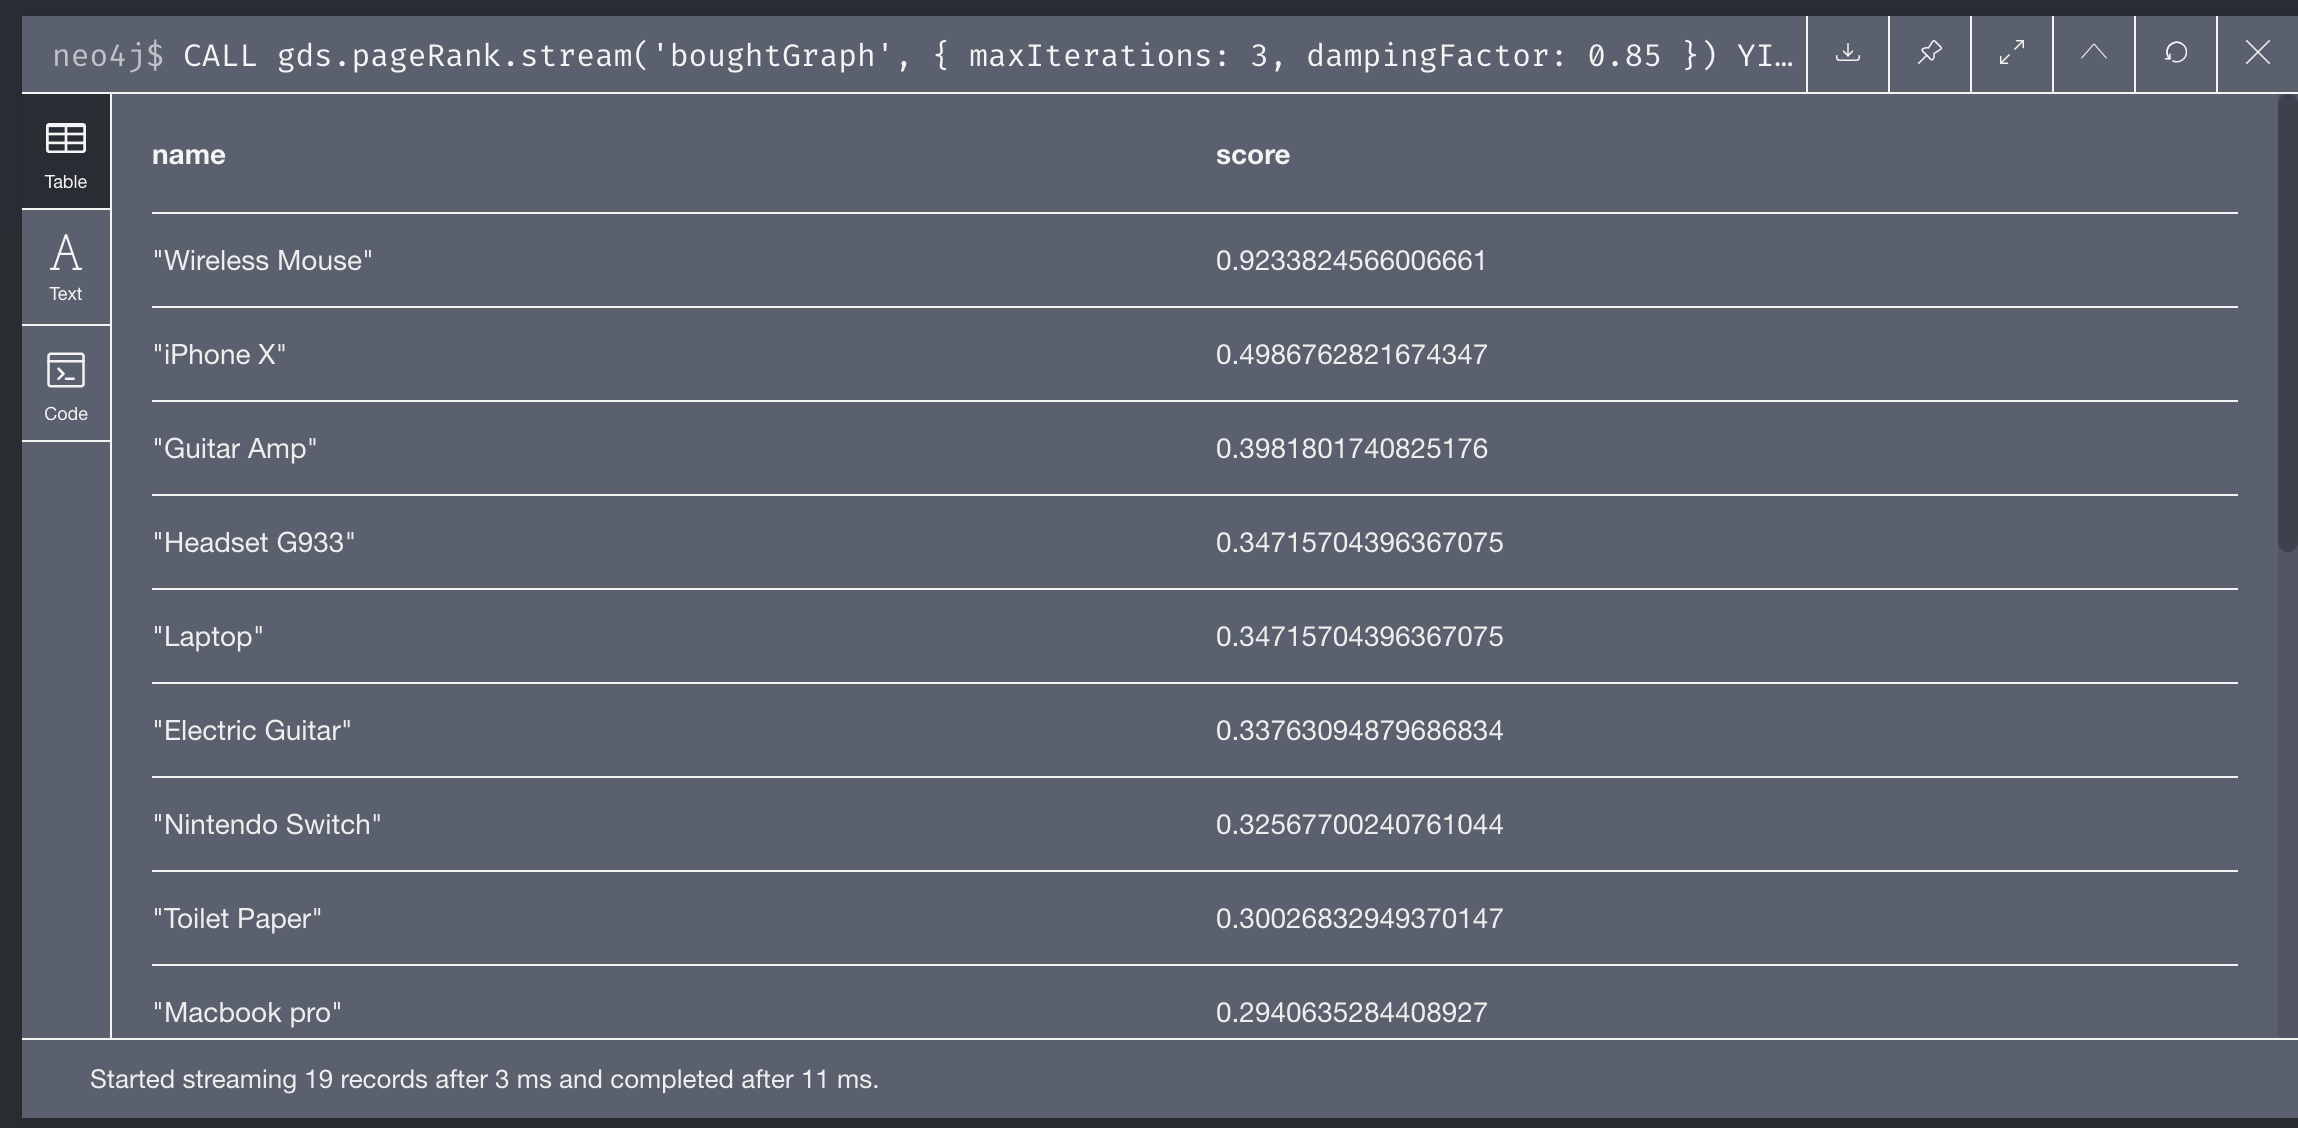
\includegraphics[width=0.95\textwidth]{img/pageRank_res_1}
	\caption{Resultaat PageRank algoritme}
	\label{fig:simplePageRankResult}
\end{figure}

\newpage
\subsection{Personalized PageRank}
\label{sec:Personalized PageRank}

Om de resultaten te baseren vanuit een bepaald startpunt, bijvoorbeeld een Customer, kan er een variant op PageRank gebruikt worden. Het algoritme zal dan starten in een bepaalde knoop (de gebruiker in kwestie) en zal op deze manier de meest relevante knopen vinden.

We gebruiken opnieuw de genoemde graaf uit de simpele PageRank, en voeren daar volgend algoritme op uit: 

\begin{lstlisting}[caption={Personalized PageRank algoritme }]
MATCH (c1:Customer {name: 'Tony'})
CALL gds.pageRank.stream('boughtGraph', {
	maxIterations: 1,
	dampingFactor: 0.85,
	sourceNodes: [c1]
	})
YIELD nodeId, score
RETURN gds.util.asNode(nodeId).name AS name, score
ORDER BY score DESC, name ASC
\end{lstlisting}

In het resultaat van deze query (Figuur \ref{fig:personalizedPageRankResult}) zien we dat de resultaten voor deze gebruiker in dezelfde lijn lopen als de algemene resultaten, maar dat er toch enkele producten bovenaan de lijst te vinden zijn die bij het gewone PageRank algoritme niet aan bod komen.

\begin{figure} [ht]
	\centering
	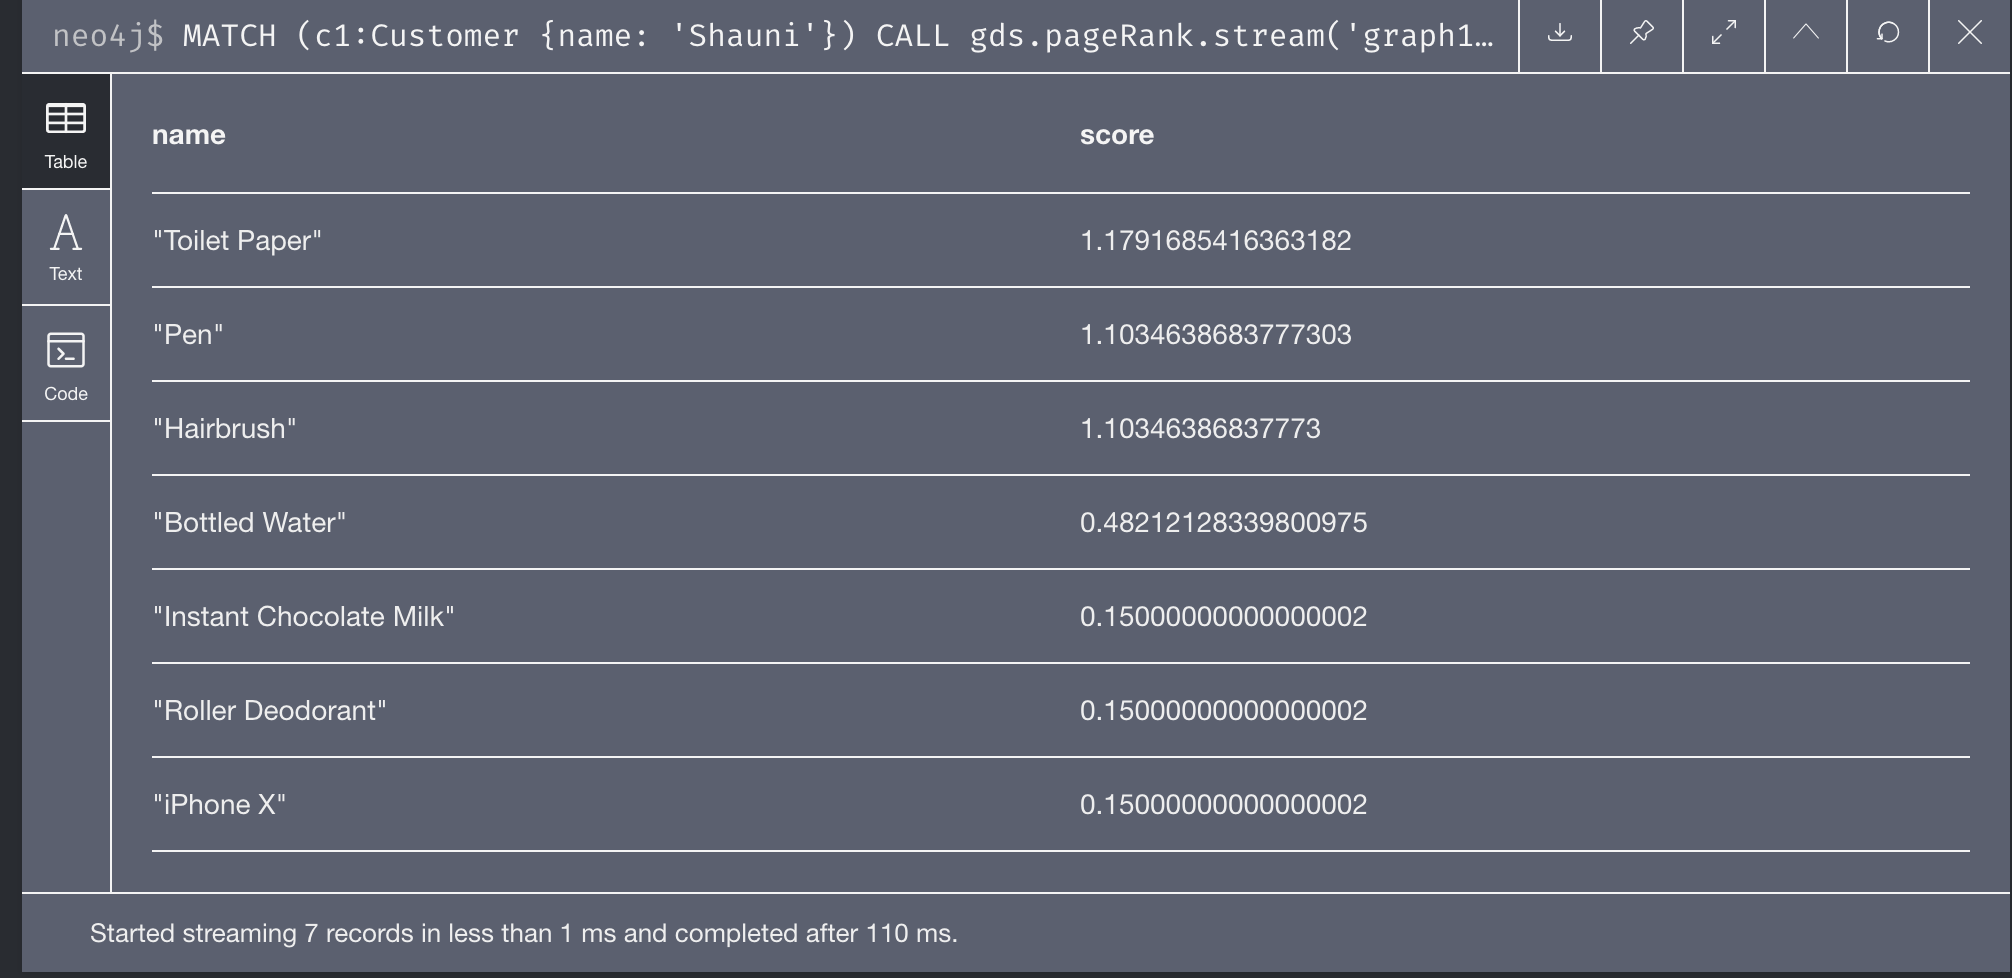
\includegraphics[width=0.95\textwidth]{img/persPageRank_res_1}
	\caption{Resultaat Personalized PageRank algoritme}
	\label{fig:personalizedPageRankResult}
\end{figure}

\newpage
\subsection{Community Detection}
\label{subsec: Community Detection}

Door het analyseren van de graaf met een community detection-algoritme kunnen groepen van gelijkaardige producten ontdekt worden. Op deze manier kan ontdekt worden welke gebruikers geïnteresseerd zijn in bepaalde groepen van producten, en kunnen er op basis van deze clusters aanbevelingen voorgesteld worden. 

Een nadeel aan deze techniek is dat deze last heeft van het cold-start probleem. Met andere woorden dat voor nieuwe gebruikers of producten, waarvoor dus nog niet bekend is tot welke cluster ze behoren of in welke clusters zij interesse hebben, nog geen correcte aanbevelingen kunnen bepaald worden.

Een voorbeeld van een community detection algoritme is het Louvain algoritme. De genoemde graaf van de uitwerking van PageRank zal opnieuw worden gebruikt voor dit algoritme.

\begin{lstlisting}[caption={ Louvain algoritme }]
CALL gds.louvain.stream('boughtGraph')
YIELD nodeId, communityId, intermediateCommunityIds
RETURN gds.util.asNode(nodeId).name AS name, communityId, intermediateCommunityIds
ORDER BY communityId DESC
\end{lstlisting}

Uit de resultaten worden enkele clusters ontdekt, deze zijn aangeduid op Figuur \ref{fig:LouvainResult}.

\begin{figure} [ht]
	\centering
	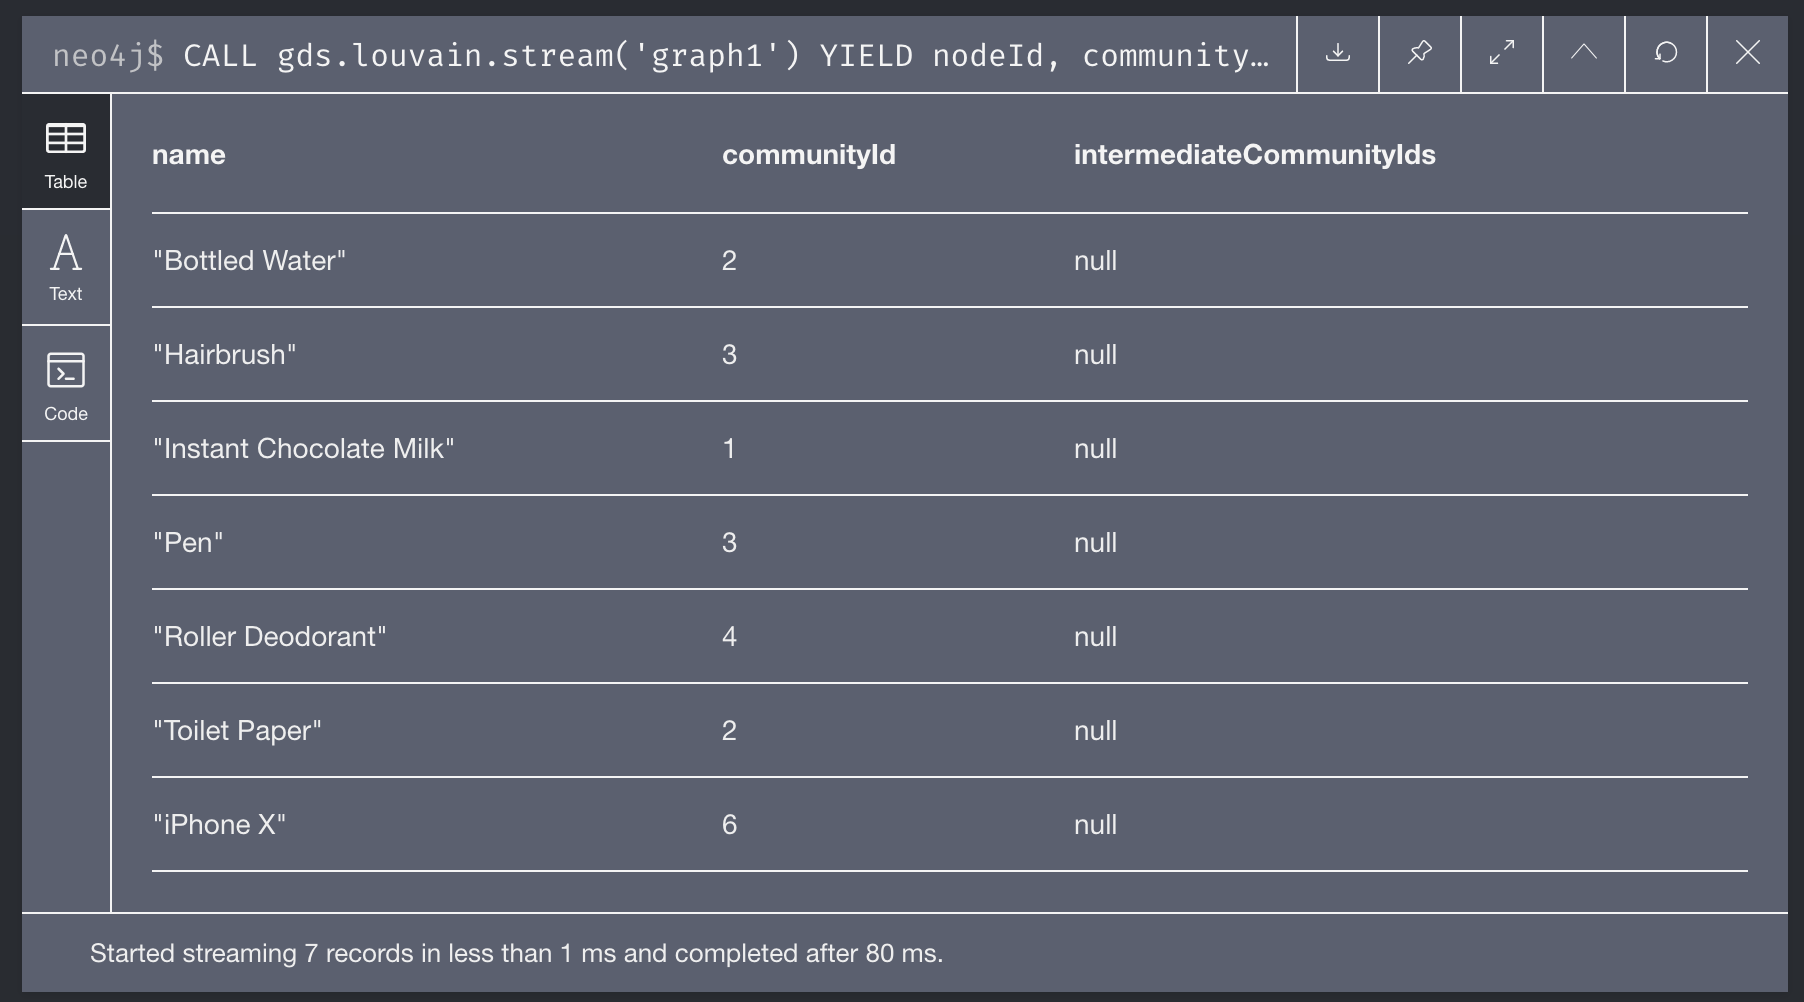
\includegraphics[width=0.95\textwidth]{img/Louvain_result}
	\caption{Resultaat Louvain algoritme}
	\label{fig:LouvainResult}
\end{figure}





% Voeg hier je eigen hoofdstukken toe die de ``corpus'' van je bachelorproef
% vormen. De structuur en titels hangen af van je eigen onderzoek. Je kan bv.
% elke fase in je onderzoek in een apart hoofdstuk bespreken.

%\input{...}
%\input{...}
%...

%%=============================================================================
%% Conclusie
%%=============================================================================

\chapter{Conclusie}
\label{ch:conclusie}

% TODO: Trek een duidelijke conclusie, in de vorm van een antwoord op de
% onderzoeksvra(a)g(en). Wat was jouw bijdrage aan het onderzoeksdomein en
% hoe biedt dit meerwaarde aan het vakgebied/doelgroep? 
% Reflecteer kritisch over het resultaat. In Engelse teksten wordt deze sectie
% ``Discussion'' genoemd. Had je deze uitkomst verwacht? Zijn er zaken die nog
% niet duidelijk zijn?
% Heeft het onderzoek geleid tot nieuwe vragen die uitnodigen tot verder 
%onderzoek?

\section{GDPR}
\label{sec: Conclusie GDPR}

Rekeninghoudend met de informatie die verkregen werd bij de literatuurstudie, kan er een antwoord geleverd worden op de onderzoeksvraag.

Indien de regels van de GDPR nageleefd worden inzake het verwerken van informatie van personen, kan er een systeem opgezet worden dat volgzaam is aan de wetgeving, en toch in staat is gepersonaliseerde zoekopdrachten uit te voeren. 

Er zal een eenduidig en ondubbelzinnig beleid moeten worden opgesteld dat de gebruiker al dan niet kan accepteren.
 Indien de gebruiker niet akkoord gaat met het beleid, of zijn informatie slechts deels ter beschikking wenst te stellen, zal hierbij rekening gehouden moeten worden dat de resultaten van zoekopdrachten in sommige gevallen minder of zelfs niet gepersonaliseerd kunnen worden.

De keuze moet hierbij volledig in handen van de gebruiker liggen, en deze moet via het beleid op de hoogte gesteld worden van de doeleinden waarvoor zijn informatie gebruikt zal worden, om zo een beslissing te maken. In de voorgestelde toepassing zal dus duidelijk vermeld moeten staan dat zijn persoonlijke informatie enkel en alleen gebruikt wordt voor het aanbieden van gepersonaliseerde zoekresultaten.

Bij het aanmaken van een account zal nogmaals een beleid moeten opgesteld worden, waarin duidelijk vermeldt staat waarvoor de data die ingevuld wordt bij de creatie van het account gebruikt zal worden. In deze toepassing zal het dus gaan over de gegevens over de woonplaats van een gebruiker, leeftijdscategorie, naam, etc.

Bijvoorbeeld voor het gebruik van de data over de woonplaats zal dus duidelijk verwoord moeten worden dat deze data gebruikt wordt voor het linken van personen binnen één gezin.

Ook zal er geen data mogen bijgehouden worden die niet relevant is voor de doelstellingen, gegevens zoals bijvoorbeeld een telefoonnummer zijn niet van belang voor onze doelstellingen, en mogen dus niet verwerkt worden. De gebruiker moet steeds in staat zijn om zijn gegevens op te vragen of deze te laten wissen, en dit moet steeds zonder onredelijke vertraging gebeuren.

Hiermee is de onderzoeksvraag beantwoordt; ja, het is mogelijk om een systeem op te stellen met een gepersonaliseerde zoekfunctie die als legaal wordt aanzien onder de wetgeving omtrent GDPR.

\section{ ElasticSearch}
\label{sec:Conclusie Elasticsearch}

Elasticsearch is zeer snel en eenvoudig in het gebruik als het gaat over het vinden van producten die relateren aan de gebruiker zelf. Uit het onderzoek bleek ook dat specifieke zoektermen en filters relatief eenvoudig te implementeren zijn.

Elasticsearch biedt ook de mogelijkheden om een graaf met de relaties tussen de verschillende documenten op te slaan, maar deze is niet zomaar verkrijgbaar, hier is een Platinum of Enterprise licentie voor vereist. Het is mogelijk om op deze manier dan toch rekening te kunnen houden met familiale relaties, alsook filters toe te passen op de zoekopdrachten.

\section{ Neo4j}
\label{sec:Conclusie Neo4j}

Neo4j, als graph databank, staat toe om gebruik te maken van alle relaties tussen de verschillende producten (nodes) om aanbevelingen te genereren. Ook zijn er enkele algoritmen reeds ingebouwd in een Graph Data Analysis plugin, die zorgen voor de meest performante werkwijze.

Qua eenvoud van implementatie is Neo4j de betere keuze, mede met dank aan het feit dat alles visueel kan toegelicht worden door simpelweg naar de graaf te kijken. 

Zowel het gebruik van de graaf, als het zoeken op basis van een tekstveld zijn mogelijk in Neo4j zonder dat hier extra kosten aan vast hangen voor licenties. 

\section{Resultaat}
\label{sec:Resultaat}

Er kan dus geconcludeerd worden dat elk van deze technieken uitblinkt in zijn eigen branche, de literatuurstudie wees ook uit dat een Knowledge Graph gebruikt kan worden om aanvullende informatie te verschaffen bij het genereren van gepersonaliseerde zoekresultaten. 

Een optie is dus om beide platformen te combineren, en elkaar te laten aanvullen. Een voorbeeld hier van is om de resultaten van een zoekalgoritme in Neo4 te combineren met de scores die gevonden werden in Elasticsearch. 

Deze ontdekking zet de weg open tot verder onderzoek in hoe deze twee platformen efficiënt samen gebruikt kunnen worden, en hoe de modellen die in dit onderzoek werden opgebouwd, verder gespecialiseerd kunnen worden om deze combinatie mogelijk te maken. 


%%=============================================================================
%% Bijlagen
%%=============================================================================

\appendix
\renewcommand{\chaptername}{Appendix}

%%---------- Onderzoeksvoorstel -----------------------------------------------

\chapter{Onderzoeksvoorstel}

Het onderwerp van deze bachelorproef is gebaseerd op een onderzoeksvoorstel dat vooraf werd beoordeeld door de promotor. Dat voorstel is opgenomen in deze bijlage.

% Verwijzing naar het bestand met de inhoud van het onderzoeksvoorstel
%---------- Inleiding ---------------------------------------------------------

\section{Introductie} % The \section*{} command stops section numbering
\label{sec:introductie}

De meeste e-commerce online platformen hebben reeds een zoekfunctie ingebouwd, maar deze is vaak beperkt tot enkel de productcatalogus. Rekening houdend met de algemene trend rond personalisering van de customer experience zou het ook aangewezen zijn om ook de search op de e-commerce site te personaliseren. Dit zou resulteren in een betere experience voor de klant en een hogere conversie voor het bedrijf. In deze bachelorproef wordt onderzocht in hoeverre de persoonlijke data van een specifieke gebruiker en contextuele data kan ingeschakeld en gecombineerd worden met de data uit de productcatalogus, om zo persoonlijke en relevante zoekresultaten te genereren. 
Met deze persoonlijke data wordt bedoeld de historische aankoopdata van de persoon zelf, maar ook bepaalde demografische data zoals geslacht, leeftijd, gezinssamenstelling, etc. De onderzoeksvraag kan dus als volgt geformuleerd worden: Welk databankmodel presteert het best om gepersonaliseerde zoekresultaten te bekomen?


%---------- Stand van zaken ---------------------------------------------------

\section{State-of-the-art}
\label{sec:state-of-the-art}

Personalized Search \autocite{Pitkow2002} verwijst naar het zoeken op het web waarbij de resultaten afhankelijk zijn van de interesses en voorkeuren van de gebruiker die verder gaan dan de query zelf. 

Personalisatie in e-commerce toepassingen biedt een groot voordeel aan bedrijven. De loyaliteit van klanten wordt veel sterker als deze gebruik maken van gepersonaliseerde features.\autocite{Telang2005} Een zoekfunctie is een voorbeeld van zo een feature.
Recommender Systems \autocite{Resnick1997} zijn aanbevelingen vanuit het systeem die rekening houden met de beschikbare informatie van gebruikers en hun voorkeuren om zo een filter te plaatsen op de informatie die weergegeven wordt. 

De studie van \textcite{Diehl2003} onderzocht het effect van gepersonaliseerde zoekresultaten op de kwaliteit van keuzes die klanten maken, en vond een positieve correlatie. De studie ontdekte dat het verlagen van search cost \autocite{Smith1999} leidde tot minder kwaliteitsvolle keuzes. De reden daarvoor is dat klanten slechtere beslissingen maken als de search cost lager ligt omdat zij minder ideale opties aangeboden krijgen. Personalized Search en Recommender System zorgen voor een enorme verbetering in de kwaliteit van de keuzes die de klant maakt, en verminderen het aantal producten die deze klant bekijkt alvorens hij/zij gevonden heeft wat hij/zij nodig heeft.

Een gevolg van gepersonaliseerde zoekopdrachten is dat we een Filter Bubble \autocite{Pariser2011} creëren. Het verlaagt de kans dat nieuwe informatie gevonden wordt doordat de resultaten van een zoekopdracht partijdig zijn en eerder wijzen naar dingen die de gebruiker reeds gezien heeft. Dit concept wordt een Filter Bubble genoemd omdat gebruikers eigenlijk geïsoleerd worden in hun eigen wereldje, waar ze enkel de informatie te zien krijgen die ze willen zien. Als we deze gebruikers met hun bubbels in groepen opdelen, verkrijgen we wel het probleem dat deze een vertekend beeld op de realiteit krijgen, zij krijgen bijvoorbeeld in het nieuws slechts het deel te zien dat voor hun interessant is. Als we deze lijn doortrekken naar de klanten van e-commerce websites, zullen zij ook slechts de merken te zien krijgen waar hun voorkeur naar uit gaat. Hierdoor verminder je de kans dat ze een nieuw merk ontdekken of een ander product uitproberen. Als we terug refereren naar de studie van \textcite{Diehl2003}, dan kunnen we afleiden dat dit een positief effect zal hebben op de klanttevredenheid.

% Voor literatuurverwijzingen zijn er twee belangrijke commando's:
% \autocite{KEY} => (Auteur, jaartal) Gebruik dit als de naam van de auteur
%   geen onderdeel is van de zin.
% \textcite{KEY} => Auteur (jaartal)  Gebruik dit als de auteursnaam wel een
%   functie heeft in de zin (bv. ``Uit onderzoek door Doll & Hill (1954) bleek
%   ...'')


%---------- Methodologie ------------------------------------------------------
\section{Methodologie}
\label{sec:methodologie}

Om de onderzoeksvraag te beantwoorden wordt er een simpele webapplicatie opgezet waar een zoekterm kan ingevoerd worden. Deze webapplicatie zal louter gebruikt worden om met behulp van een tekstveld een query op een databank uit te voeren. Ook worden er twee databankmodellen ontworpen, een model dat gebruik maakt van Neo4j (Graph databank platform), en een model dat gebruik maakt van Elasticsearch (OLAP databank platform) en Kibana om de resultaten te visualiseren. Graph is een databankstructuur van het type NoSQL, dit wil algemeen zeggen dat ze geen gebruik maken van SQL. Bij Graph databanken worden gegevens voorgesteld door een geheel van entiteiten en verbindingen, alsook vrije relaties tussen deze entiteiten. Kortom is dit, zoals de naam al laat vermoeden, een graaf. OLAP is de afkorting voor Online Analytical Processing, dit is een technologie die geoptimaliseerd is voor het uitvoeren van query's en rapporten in plaats van transacties. Deze zullen elk met hun eigen API communiceren, en in beide modellen wordt dezelfde gebruiker- en productdata ingevoerd. Bij het opstellen van de modellen wordt mogelijk al duidelijk of één van de modellen niet in staat zal zijn om dezelfde functionaliteiten te hebben als het andere, en dan zal moeten afgewogen worden of de voordelen van het ene model opwegen tegenover het andere model. Als beide modellen dezelfde functionaliteit kunnen bereiken, wordt er bekeken welke het meest performante is. Mogelijks zou het ook haalbaar zijn om beide manieren te combineren op voorwaarde dat de responstijd binnen de acceptabele norm valt.


%---------- Verwachte resultaten ----------------------------------------------
\section{Verwachte resultaten}
\label{sec:verwachte_resultaten}

Er wordt verwacht dat er ofwel een duidelijk verschil merkbaar is in performantie tussen de twee verschillende modellen. Mogelijk is dat één van de twee modellen totaal niet haalbaar is om efficiënt een link mee te leggen tussen bijvoorbeeld familieleden, in dit geval bekijken we of het mogelijk is deze twee modellen samen uit te voeren, als dit een resultaat biedt dat binnen de norm valt qua performantie, dan is dit ook een mogelijke oplossing.
 Het kan zich ook voordoen dat beide modellen vrij performant en efficiënt de query's kunnen verwerken, in dit geval worden de voor- en nadelen alsook de moeilijkheidsgraad van implementatie afgewogen.


%---------- Verwachte conclusies ----------------------------------------------
\section{Verwachte conclusies}
\label{sec:verwachte_conclusies}

Er wordt verwacht dat het Graph model makkelijker te implementeren zal zijn en beter zal presteren als we rekening willen houden met het aankoopgedrag van vrienden en familie. Indien dit ook mogelijk is bij een OLAP-model, verwachten we dat Graph nog steeds beter zal presteren. Indien we hier geen rekening mee houden zal het OLAP-model beter presteren, aangezien dit model aangepast is aan grote hoeveelheden data waar complexe zoekopdrachten op kunnen uitgevoerd worden.




%%---------- Andere bijlagen --------------------------------------------------
% TODO: Voeg hier eventuele andere bijlagen toe
%\input{...}

%%---------- Referentielijst --------------------------------------------------

\printbibliography[heading=bibintoc]

\end{document}
